\graphicspath{{./figures/}}
\title{pipelining}
\date{}
\usepackage{pgfplots}
\begin{document}
\usepgflibrary{shapes.gates.logic.mux}
\usepgfplotslibrary{fillbetween}
\usetikzlibrary{calc,chains,shapes.misc,shapes.callouts,shapes.geometric,shapes.gates.logic.US,circuits.logic.US}
\usetikzlibrary{arrows.meta,chains,positioning,matrix,fit}


\ifdefined\NOBEAMER\else
\newcommand<>{\mathHL}[1]{%
\alt#2{
\text{\colorbox{green!20}{\ensuremath{#1}}}%
}{
\text{\colorbox{white!20}{\ensuremath{#1}}}%
}%
}
\fi

\makeatletter
\pgfdeclareshape{myregister}%
{
    \inheritsavedanchors[from=rectangle]
    \inheritanchorborder[from=rectangle]
    \inheritanchor[from=rectangle]{center}
    \inheritanchor[from=rectangle]{north}
    \inheritanchor[from=rectangle]{south}
    \inheritanchor[from=rectangle]{west}
    \inheritanchor[from=rectangle]{east}
    \inheritanchor[from=rectangle]{north east}
    \inheritanchor[from=rectangle]{north west}
    \inheritanchor[from=rectangle]{south east}
    \inheritanchor[from=rectangle]{south west}
    \inheritbackgroundpath[from=rectangle]
    \saveddimen{\halfbaselength}{%
         \pgf@x=0.5\wd\pgfnodeparttextbox
         % get xsep
         \pgfmathsetlength\pgf@xc{\pgfkeysvalueof{/pgf/inner xsep}}%
         \advance\pgf@x by \pgf@xc%
         % get \ht of textbox, add to baselength 
         \advance\pgf@x by \wd\pgfnodeparttextbox
         % get minimum width
         \pgfmathsetlength\pgf@xb{\pgfkeysvalueof{/pgf/minimum width}}%
         \divide\pgf@xb by 2
         \ifdim\pgf@x<\pgf@xb%
             % yes, too small. Enlarge...
             \pgf@x=\pgf@xb%
         \fi%
     }
    \backgroundpath{
        \pgfpathrectanglecorners{\southwest}{\northeast}
        \southwest \pgf@xa=\pgf@x \pgf@ya=\pgf@y 
        \pgf@yb=\pgf@ya
        \northeast \pgf@xb=\pgf@x %\pgf@yb=\pgf@y
        \pgf@xc = \pgf@xa
        \advance\pgf@xc by \halfbaselength
        \pgf@yc=\pgf@ya
        \advance\pgf@yc by \halfbaselength
        \pgfpathmoveto{\pgfpoint{\pgf@xa}{\pgf@ya}}
        \pgfpathlineto{\pgfpoint{\pgf@xc}{\pgf@yc}}
        \pgfpathlineto{\pgfpoint{\pgf@xb}{\pgf@yb}}
        \pgfpathclose
    }
}
\makeatother

\newcommand{\rA}{\it rA}
\newcommand{\rB}{\it rB}
\newcommand{\V}{\it V}
\newcommand{\D}{\it D}
\newcommand{\fn}{\it fn}
\newcommand{\Dest}{\it Dest}
\newcommand{\cc}{\it cc}
\tikzset{extra box/.style={},
         extra box opcode/.style={},
         extra box fn/.style={},
         extra box cc/.style={},
         extra box register/.style={},
         extra box immediate/.style={},
         extra box shorter width/.style={},
         extra box fake/.style={},
         }
\newcommand{\instrEncodingStyles}{
\tikzset{
    empty box/.style={text height=1ex,text depth=.4ex,font=\tt\fontsize{9}{10}\selectfont},
    box/.style={draw,rectangle,thick,empty box,extra box,align=center},
    opcode/.style={box,fill=blue!40!white,extra box opcode},
    secondOpcode/.style={box,fill=violet!40!white},
    secondOpcodeFN/.style={secondOpcode,extra box fn},
    secondOpcodeCC/.style={secondOpcode,extra box cc},
    literal/.style={box,fill=white!90!black},
    register/.style={box,fill=red!40!white,extra box register},
    fake/.style={empty box,pattern color=red!40!white,pattern=north west lines,inner sep=-1pt,extra box fake},
    immediate/.style={box,fill=green!40!white,extra box immediate},
    immediateLabel/.style={box,fill=green!40!white,extra box immediate,label={center:\fontsize{9}{10}\selectfont##1}},
}
}
\newcommand{\ccify}[2]{\begin{tikzpicture}[baseline]\node[anchor=base,secondOpcodeCC,text width=.35cm,inner xsep=0pt,inner sep=2pt,outer sep=0pt]{#1};\end{tikzpicture}}
\newcommand{\fnify}[1]{\begin{tikzpicture}[baseline]\node[anchor=base,secondOpcodeFN,text width=.35cm,inner xsep=0pt,inner sep=2pt,outer sep=0pt]{#1};\end{tikzpicture}}
\newcommand{\fnifyWide}[1]{\begin{tikzpicture}[baseline]\node[anchor=base,secondOpcodeFN,inner xsep=0pt,inner sep=2pt,outer sep=0pt,dashed]{#1};\end{tikzpicture}}
\newcommand{\opify}[1]{\begin{tikzpicture}[baseline]\node[anchor=base,opcode,text width=.35cm,inner xsep=0pt,inner sep=2pt,outer sep=0pt]{#1};\end{tikzpicture}}
\newcommand{\opifyWide}[1]{\begin{tikzpicture}[baseline]\node[anchor=base,opcode,inner xsep=0pt,inner sep=2pt,outer sep=0pt]{#1};\end{tikzpicture}}
\newcommand{\literalify}[1]{\begin{tikzpicture}[baseline]\node[anchor=base,literal,text width=.35cm,inner xsep=0pt,inner sep=2pt,outer sep=0pt]{#1};\end{tikzpicture}}
\newcommand{\immedify}[1]{\begin{tikzpicture}[baseline]\node[anchor=base,immediate,inner xsep=0pt,inner sep=2pt,outer sep=0pt]{#1};\end{tikzpicture}}
\newcommand{\rnify}[1]{\begin{tikzpicture}[baseline]\node[anchor=base,register,text width=.35cm,inner xsep=0pt,inner sep=2pt,outer sep=0pt]{#1};\end{tikzpicture}}
\newcommand{\rnifyWide}[1]{\begin{tikzpicture}[baseline]\node[anchor=base,register,inner xsep=0pt,inner sep=2pt,outer sep=0pt,dashed]{#1};\end{tikzpicture}}

\newcommand{\movq}{{\keywordstyle movq}\xspace}
\newcommand{\rmmovq}{{\keywordstyle rmmovq}\xspace}
\newcommand{\mrmovq}{{\keywordstyle mrmovq}\xspace}
\newcommand{\addq}{{\keywordstyle addq}\xspace}
\newcommand{\subq}{{\keywordstyle subq}\xspace}
\newcommand{\xorq}{{\keywordstyle xorq}\xspace}
\newcommand{\andq}{{\keywordstyle andq}\xspace}
\newcommand{\asmj}{{\keywordstyle jmp}\xspace}
\newcommand{\call}{{\keywordstyle call}\xspace}
\newcommand{\halt}{{\keywordstyle halt}\xspace}
\newcommand{\ret}{{\keywordstyle ret}\xspace}
\newcommand{\nop}{{\keywordstyle nop}\xspace}
\newcommand{\irmovq}{{\keywordstyle irmovq}\xspace}
\newcommand{\rrmovq}{{\keywordstyle rrmovq}\xspace}
\newcommand{\jmp}{{\keywordstyle jmp}\xspace}

\tikzset{
    hReg/.style={draw,myregister,minimum width=.4cm,minimum height=2cm,label={[font=\small,align=center]-90:#1}},
    hhReg/.style={draw,myregister,minimum width=.3cm,minimum height=5.5cm,label={[font=\small,align=center]-90:#1}},
    horizReg/.style={draw,myregister,rotate=-90,minimum width=.1cm,minimum height=1cm,label={[font=\small,align=center,fill=white]90:#1}},
    wReg/.style={draw,myregister,minimum width=2cm,minimum height=.4cm,label={[font=\small]-90:#1}},
    hRegSmall/.style={draw,myregister,minimum height=.6cm,minimum width=.2cm,label={[font=\small,inner sep=.5mm,align=center]-90:#1}},
    hRegT/.style={hRegSmall,minimum height=.4cm},
    mem/.style={draw,rectangle,minimum height=1.5cm,minimum width=1cm,inner sep=4pt,align=center,font=\small},
    memBig/.style={draw,rectangle,minimum height=3cm,minimum width=3cm,align=center,font=\small},
    regFile/.style={draw,rectangle,minimum height=4cm,minimum width=2cm,align=center,font=\small},
    ll/.style={font=\scriptsize},
    a/.style={-{Latex[length=5pt,width=3pt]},thick},
    aR/.style={{Latex[length=5pt,width=3pt]}-,thick},
    aN/.style={thick},
    aa/.style={-{Latex[length=5pt,width=3pt]},line width=1.2pt},
    aaR/.style={{Latex[length=5pt,width=3pt]}-,line width=1.2pt},
    aaN/.style={line width=1.2pt},
    b/.style={-{Latex[length=2pt,width=2pt]}},
    bN/.style={thin},
    bb/.style={line width=.5pt,-{Latex[length=2pt,width=2pt]}},
    bbR/.style={line width=.5pt,{Latex[length=2pt,width=2pt]}-},
    bR/.style={{Latex[length=2pt,width=2pt]}-},
    global scale/.style={scale=#1,every node/.style={scale=#1}},
    %logicBlock/.style={draw,cloud,cloud puffs=13.7,inner sep=0pt,cloud ignores aspect,align=center,draw},
    logicBlock/.style={draw,rectangle,inner sep=1pt,align=center,draw,fill=blue!20},
    logicBlockS/.style={draw,rectangle,inner sep=1pt,align=center,draw,fill=blue!20,font=\small},
    control/.style={dashed,color=blue!60},
    logicFill/.style={fill=blue!20},
    offsetBox/.style={align=left,font=\small,draw=blue!60!black,line width=2pt,rectangle}
}

\tikzset{
    bookLabel/.style={color=red!60!black,font=\small\bfseries,outer sep=0pt,inner sep=1pt,fill=white},
    imemPcPre/.style={invisible},
    imemPc/.style={},
    instrRegs/.style={},
    instrRegsPre/.style={invisible},
    instrRegsSplitOut/.style={invisible},
    instrRegsSplitImmed/.style={instrRegsSplitOut},
    instrRegsRS1/.style={instrRegs},
    instrRegsMux/.style={instrRegs},
    instrRegsMuxRS2/.style={instrRegsMux},
    instrRegsMuxRS3/.style={instrRegsMux},
    instrRegsMuxRS3F/.style={instrRegsMuxRS3},
    instrRegsMuxRS4/.style={instrRegsMux},
    instrRegsRS34Loop/.style={invisible},
    instrRegsNoMux/.style={invisible},
    instrRegsNoMuxRS2/.style={instrRegsNoMux},
    instrRegsNoMuxRS3/.style={instrRegsNoMux},
    instrRegsNoMuxRS4/.style={instrRegsNoMux},
    instrRegsPreSingle/.style={invisible},
    regsLogic/.style={},
    regsLogicMux/.style={regsLogic},
    regsLogicMuxA/.style={regsLogicMux},
    regsLogicMuxB/.style={regsLogicMux},
    regsLogicNoMux/.style={invisible},
    regsLogicNoMuxA/.style={regsLogicNoMux},
    regsLogicNoMuxB/.style={regsLogicNoMux},
    logicDmem/.style={},
    logicDmemMux/.style={logicDmem},
    logicDmemNoMux/.style={invisible},
    dmemWB/.style={},
    dmemWBFromMem/.style={dmemWB},
    dmemWBvalENoMux/.style={dmemWB},
    dmemWBvalELoop/.style={invisible},
    dmemWBvalEMux/.style={invisible},
    dmemOutToPC/.style={dmemWB},
    dmemPC/.style={},
    dmemPCMux/.style={dmemPC},
    dmemPCNoMux/.style={invisible},
    pcDecode/.style={},
    isStatReg/.style={hRegSmall=#1},
    isStat/.style={invisible},
    dmemNorm/.style={},
    dmemInputLabel/.style={dmemNorm},
    dmemLabel/.style={invisible},
    dmemPre/.style={invisible},
    dmemPreSingle/.style={invisible},
    regNorm/.style={},
    regNormLabel/.style={},
    regNormLabelE/.style={regNormLabel},
    regNormLabelM/.style={regNormLabel},
    regPre/.style={},
    regPreSingle/.style={},
    ccsNorm/.style={invisible},
    smallLabel/.style={font=\scriptsize,inner sep=1pt,outer sep=0pt},
    smallerLabel/.style={font=\tiny,inner sep=1pt,outer sep=0pt},
    pcStyle/.style={},
    wbPCLine/.style={},
    aluOpExplain/.style={regsLogic},
    funcOpExplain/.style={logicDmem},
    muxDst/.style={},
}
\newcommand{\instrEncodingSubTable}[3]{
\matrix[matrix of nodes,
    column sep=-2\pgflinewidth,
    row sep=2.5pt,
    nodes={empty box,text width=.35cm,inner xsep=0pt, inner sep=2pt,outer sep=0pt},
    column 1/.style={nodes={font=\tt\fontsize{9}{10}\selectfont,text width=3.5cm}},
    column 6/.style={nodes={extra box shorter width}},
    column 7/.style={nodes={extra box shorter width}},
    column 8/.style={nodes={extra box shorter width}},
    column 9/.style={nodes={extra box shorter width}},
    column 10/.style={nodes={extra box shorter width}},
    column 11/.style={nodes={extra box shorter width}},
    column 12/.style={nodes={extra box shorter width}},
    column 13/.style={nodes={extra box shorter width}},
    column 14/.style={nodes={extra box shorter width}},
    column 15/.style={nodes={text width=.2cm,extra box shorter width}},
    column 16/.style={nodes={text width=.2cm,extra box shorter width}},
    column 17/.style={nodes={text width=.2cm,extra box shorter width}},
    column 18/.style={nodes={text width=.2cm,extra box shorter width}},
    column 19/.style={nodes={text width=.2cm,extra box shorter width}},
    column 20/.style={nodes={text width=.2cm,extra box shorter width}},
    column 21/.style={nodes={text width=.2cm,extra box shorter width}},
#1,
] (#2) {#3}}

\newcommand{\var}[1]{\ensuremath{\text{#1}}}
\newcommand{\icode}{\var{icode}}
\newcommand{\ifun}{\var{ifun}}
\newcommand{\vrA}{\var{rA}}
\newcommand{\vrB}{\var{rB}}
\newcommand{\valP}{\var{valP}}
\newcommand{\valA}{\var{valA}}
\newcommand{\valB}{\var{valB}}
\newcommand{\valC}{\var{valC}}
\newcommand{\valE}{\var{valE}}
\newcommand{\valM}{\var{valM}}
\newcommand{\PC}{\var{PC}}
\newcommand{\srcA}{\var{srcA}}
\newcommand{\srcB}{\var{srcB}}
\newcommand{\dstE}{\var{dstE}}
\newcommand{\dstM}{\var{dstM}}
\newcommand{\aluA}{\var{aluA}}
\newcommand{\aluB}{\var{aluB}}
\newcommand{\pcMemDist}{2.cm}
\newcommand{\imemRegsDist}{3.5cm}
\newcommand{\regAluDist}{1.25cm}
\newcommand{\regMemDist}{3cm}
\newcommand{\regMuxDmemDist}{1.5cm}
\newcommand{\regReadOffset}{0cm}
\newcommand{\dstMuxDelta}{2.5mm}
\newcommand{\ilenOffset}{0cm}
\newcommand{\pcLabel}{PC}
\newcommand{\prePcDist}{2.5mm}
\newcommand{\regRegLabelDist}{1.5cm}
\newcommand{\regBDist}{.4cm}

\newcommand{\circuitStateToALU}{
        \node[hReg=\pcLabel,pcStyle] (pc) {};
        \node[mem,right=\pcMemDist of pc,font=\scriptsize] (imem) {Instr. \\ Mem.};
        \coordinate (imemData) at (imem.east);
        \coordinate (imemAddr) at (imem.west);
        \begin{scope}[regNorm]
            \node[regFile,right=\imemRegsDist of imem,label={[label distance=1pt,inner sep=0pt]\small register file}] (regs) {};
            \coordinate (regSelect1) at ($(regs.north west) - (0cm, .5cm)$);
            \coordinate (regSelect2) at ($(regs.north west) - (0cm, 1cm)$);
            \coordinate (regSelect3) at ($(regs.north west) - (0cm, 1.5cm)$);
            \coordinate (regSelect4) at ($(regs.north west) - (0cm, 2cm)$);
            \coordinate (regWriteIn1) at ($(regs.north west) - (0cm, 3.0cm)$);
            \coordinate (regWriteIn2) at ($(regs.north west) - (0cm, 3.5cm)$);
            \coordinate (regRead1) at ($(regs.north east) - (0cm, .4cm)$);
            \coordinate (regRead2) at ($(regs.north east) - (0cm, .4cm) - (0cm, \regBDist)$);
            %\node[ll,below left=0pt of regWriteIn,outer sep=1pt,inner sep=0pt] {data};
        \end{scope}
        \begin{scope}[regNormLabel]
            \node[smallLabel,right=0mm of regSelect1] (srcALabel) {\srcA};
            \node[smallLabel,right=0mm of regSelect2] (srcBLabel) {\srcB};
            \node[smallLabel,left=0mm of regRead1] {R[\srcA]};
            \node[smallLabel,left=0mm of regRead2] {R[\srcB]};
        \end{scope}[regNormLabel]

        \begin{scope}[regNormLabelE]
            \node[smallLabel,right=0mm of regSelect4] (dstELabel) {\dstE};
            \node[smallLabel,right=0mm of regWriteIn2] {next R[\dstE]};
        \end{scope}
        \begin{scope}[regNormLabelM]
            \node[smallLabel,right=0mm of regSelect3] (dstMLabel) {\dstM};
            \node[smallLabel,right=0mm of regWriteIn1] {next R[\dstM]};
        \end{scope}
}

\newcommand{\circuitState}{
        \circuitStateToALU
        \begin{scope}[dmemNorm]
            \node[mem,right=\regMemDist of regs,minimum width=1.3cm] (dmem) {};
            \node[dmemLabel,align=center] at (dmem) {Data\\Mem.};
            \coordinate (dmemIn) at (dmem.west);
            \coordinate (dmemInHigh) at ([yshift=.3cm]dmem.west);
            \coordinate (dmemInLow) at ([yshift=-.3cm]dmem.west);
            \coordinate (dmemDataOut) at (dmem.east);
        \end{scope}
        \begin{scope}[ccsNorm]
            \node[below=1cm of dmem,hRegSmall=ZF/SF] (ccs) {};
        \end{scope}
        \begin{scope}[isStat]
            \node[isStatReg=Stat,below=.25cm of dmem] (Stat) {};
        \end{scope}
}
\newcommand{\circuitStatePre}{
        \begin{scope}[imemPcPre]
            \draw[thick,latex-] (pc.west) -- +(-.5cm,0cm);
            \draw[thick,latex-] (imemAddr) -- +(-.3cm,0cm);
            \draw[thick,-latex] (pc.east) -- +(.3cm,0cm);
            \draw[thick,-latex] (imemData) -- +(.5cm,0cm);
        \end{scope}
        \begin{scope}[regPre]
            \draw[a,-latex,double] (regRead1) -- +(.5cm,0cm);
            \draw[thick,double,latex-] (regWriteIn1) -- +(-.5cm,0cm);
        \end{scope}
        \begin{scope}[regPreSingle]
            \draw[a,-latex] (regRead1) -- +(.5cm,0cm);
            \draw[thick,latex-] (regWriteIn1) -- +(-.5cm,0cm);
            \draw[a,-latex] (regRead2) -- +(.5cm,0cm);
            \draw[thick,latex-] (regWriteIn2) -- +(-.5cm,0cm);
        \end{scope}
        \begin{scope}[instrRegsPre]
            %\foreach \x in {regSelect1,regSelect2} {
            %    \draw[latex-] (\x) -- +(-.5cm,0cm);
            %}
            \draw[b,latex-,double] (regSelect1) -- +(-.5cm,0cm);
        \end{scope}
        \begin{scope}[instrRegsPreSingle]
            \foreach \x in {regSelect1,regSelect2,regSelect3,regSelect4} {
                \draw[latex-] (\x) -- +(-.5cm,0cm);
            }
        \end{scope}
        \begin{scope}[dmemPre]
            \draw[thick,-latex] (dmemDataOut) -- +(.5cm,0cm);
            \draw[thick,double,latex-] (dmemIn) -- +(-.5cm,0cm);
        \end{scope}
        \begin{scope}[dmemPreSingle]
            \draw[thick,-latex] (dmemDataOut) -- +(.5cm,0cm);
            \draw[thick,latex-] (dmemInHigh) -- +(-.5cm,0cm);
            \draw[thick,latex-] (dmemInLow) -- +(-.5cm,0cm);
        \end{scope}
}
\newcommand{\dmemInput}{
    \begin{scope}[dmemInputLabel]
        \node[smallLabel,right=0mm of dmemInHigh] {Data in};
        \node[smallLabel,right=0mm of dmemInLow] {Addr in};
        \node[smallLabel,left=0mm of dmemDataOut] {Data out};
    \end{scope}
}

\newcommand{\circuitConnectDetail}{
    \dmemInput

    % PC/IMEM
    \begin{scope}[imemPc]
        \draw[a] (pc.east) -- (imemAddr);
    \end{scope}

    % IMEM/REGISTERS
    \begin{scope}[instrRegs]
        \coordinate (split) at ([xshift=1cm]imemData);
        \coordinate (splitIcode) at ([xshift=.15cm]imemData);
        \coordinate (splitImmed) at ([xshift=.25cm]imemData);
        \coordinate (splitrA) at ([xshift=.5cm]imemData);
        \coordinate (splitrB) at ([xshift=.75cm]imemData);
        \draw[line width=1.5pt] (imemData) -- (splitIcode);
        \draw[line width=1.25pt] (imemData) -- (splitImmed);
        \coordinate (aboveRegFile) at ([yshift=.5cm]regs.north);
        \coordinate (furtherAboveRegFile) at ([yshift=.75cm]regs.north);

        \begin{scope}[instrRegsSplitOut]
            \draw[b] (splitrA) |- ([xshift=-1cm]regSelect1);
            \draw[b] (splitrB) |- ([xshift=-1cm]regSelect2);
        \end{scope}
        \begin{scope}[instrRegsSplitImmed]
            \draw[a] (splitImmed) |- (aboveRegFile) node[right,bookLabel] {valC};
        \end{scope}

        \begin{scope}[instrRegsRS1]
            \draw[b] (splitrA) |- (regSelect1);
        \end{scope}

        \begin{scope}[instrRegsNoMuxRS2]
           \draw[b] (splitrB) |- (regSelect2);
        \end{scope}
        \begin{scope}[instrRegsNoMuxRS3]
            \draw[b] (splitrA) |- (regSelect3);
        \end{scope}
        \begin{scope}[instrRegsNoMuxRS4]
            \draw[b] (splitrB) |- (regSelect4);
        \end{scope}

        \draw[line width=.75pt] (imemData) -- (splitrA);
        \draw[line width=0.5pt] (splitrA) -- (splitrB);
        
            \begin{scope}[instrRegsMuxRS3]
                \node[draw,minimum height=2cm,minimum width=1.25cm,left=\dstMuxDelta of regSelect3,mux,inputs={nn},global scale=0.25] (muxDstM) {};
                \draw[thin] (splitrA |- muxDstM.input 1) -- ([xshift=-2pt]splitrB |- muxDstM.input 1);
                \draw[b] ([xshift=2pt]splitrB |- muxDstM.input 1) -- (muxDstM.input 1);
                \draw[b] (muxDstM.output) -- (regSelect3);
                %\draw[bR] (muxDstM.input 3) -| (splitrB);
            \end{scope}
            \begin{scope}[instrRegsMuxRS3F]
                \draw[bR] (muxDstM.input 2) -- ++(180:2.5mm) node[left,inner sep=0pt,font=\tiny\tt] {0xF};
            \end{scope}
            \begin{scope}[instrRegsMuxRS4]
                \node[draw,minimum height=2cm,minimum width=1.25cm,left=\dstMuxDelta of regSelect4,mux,inputs={nnn},global scale=0.25] (muxDstE) {};
                \draw[b] (muxDstE.output) -- (regSelect4);
                \draw[bR] (muxDstE.input 2) -- ++(180:2.5mm) node[left,inner sep=0pt,font=\tiny\tt] {0xF};

                \draw[b] (splitrB) |- (muxDstE.input 1);
                \draw[bR] (muxDstE.input 3) -- ++(-.25cm,-.4mm) node[left,font=\tiny\tt,inner sep=0pt] {\%rsp};
            \end{scope}

            \begin{scope}[instrRegsMuxRS2]
                \node[draw,mux,minimum height=1.5cm,minimum width=0.5cm,global scale=0.25,inputs={nn},anchor=output,minimum height=1cm] (muxSrcB) at ([xshift=-.25cm]regSelect2) {};

                \draw[b] (muxSrcB.output) -- (regSelect2);
                \draw[b] (splitrB) |- (muxSrcB.input 1);
                \draw[bR] (muxSrcB.input 2) -- ++(-.25cm,-.25mm) node[left,font=\tiny\tt,inner sep=0pt] {\%rsp};
            \end{scope}

            \begin{scope}[instrRegsRS34Loop]
                \node[draw,minimum height=2cm,minimum width=1cm,mux,inputs={nnn},global scale=0.25,muxDst] (muxDstEAbove)
                    at ([yshift=1cm]regs.north) {};
                \node[draw,minimum height=2cm,minimum width=1cm,mux,inputs={nn},global scale=0.25,muxDst] (muxDstMAbove)
                    at ([yshift=1.5cm]regs.north) {};

                \coordinate (splitOffRBLoop) at ([xshift=-1cm]regSelect2 |- muxSrcB.input 1);
                \draw[bN] ([xshift=-1.25cm]regSelect1) |- ([xshift=-1.25cm,yshift=-2pt]regSelect1 |- aboveRegFile);
                \draw[b] ([xshift=-1.25cm,yshift=2pt]regSelect1 |- aboveRegFile) |- (muxDstMAbove.input 2);
                \draw[bN] (splitOffRBLoop) -- ([yshift=-2pt]splitOffRBLoop |- regSelect1);
                \draw[bN] ([yshift=2pt]splitOffRBLoop |- regSelect1) -- ([yshift=-2pt]splitOffRBLoop |- aboveRegFile);
                %\draw[b] ([yshift=2pt]splitOffRBLoop |- aboveRegFile) |- (muxDstMAbove.input 3);
                \draw[bR] (muxDstMAbove.input 1) -- ++(180:2.5mm) node[left,inner sep=0pt,font=\tiny\tt] {0xF};

                \draw[bR] (muxDstEAbove.input 1) -- ++(180:2.5mm) node[left,inner sep=0pt,font=\tiny\tt] {0xF};
                \draw[bR] (muxDstEAbove.input 2) -- ++(180:2.5mm) node[left,inner sep=0pt,font=\tiny\tt] {\%rsp};
                \draw[b] ([yshift=2pt]splitOffRBLoop |- aboveRegFile) |- (muxDstEAbove.input 3);

                \coordinate (dstMUpperRightCorner) at ([xshift=.5cm,yshift=2cm]dmem.north east);
                \coordinate (dstEUpperRightCorner) at ([xshift=.4cm,yshift=1.9cm]dmem.north east);
                \coordinate (dstMLowerRightCorner) at ([xshift=.5cm,yshift=-2.3cm]dmem.south east);
                \coordinate (dstELowerRightCorner) at ([xshift=.4cm,yshift=-2.2cm]dmem.south east);
                \coordinate (dstELeft) at ([xshift=-.75cm]regs.west);
                \coordinate (dstMLeft) at ([xshift=-1cm]regs.west);
                \coordinate (badLineHeight) at ([yshift=-.75cm]regs.south west);
                \draw[bN] (muxDstMAbove.output) -- ++(0.35cm, 0cm) |- (dstMUpperRightCorner) -- (dstMLowerRightCorner)
                    -| ([yshift=-2pt]dstMLeft |- badLineHeight);
                \draw[b] ([yshift=2pt]dstMLeft |- badLineHeight) |- (regSelect3);
                \draw[bN] (muxDstEAbove.output) -- ++(0.25cm, 0cm) |- (dstEUpperRightCorner) -- (dstELowerRightCorner)
                    -| ([yshift=-2pt]dstELeft |- badLineHeight);
                \draw[b] ([yshift=2pt]dstELeft |- badLineHeight) |- (regSelect4);
            \end{scope}
        
        \node[left=\regRegLabelDist of regSelect1,fill=white,font=\tiny,inner sep=1pt,outer sep=0pt] (vrALabel) {\vrA};
        \node[left=\regRegLabelDist of regSelect2,fill=white,font=\tiny,outer sep=0pt,inner sep=1pt] (vrBLabel) {\vrB};
    \end{scope}


    % REGISTERS/ALU
    % + ALU component
    \begin{scope}[regsLogic]
        \node[right=\regAluDist of regs,minimum height=1cm,minimum width=.75cm,logicBlock,label={[label distance=1pt,inner sep=0pt]\small ALU}] (alu) {};
        \coordinate (aluTop) at ([yshift=-2mm]alu.north west);
        \coordinate (aluBottom) at ([yshift=2mm]alu.south west);
        \node[smallerLabel,right=0mm of aluTop] {\aluA};
        \node[smallerLabel,right=0mm of aluBottom] {\aluB};
        \node[smallerLabel,left=0mm of alu.east] {\valE};
        \coordinate (afterAlu) at ([xshift=1mm]alu.east);

        \coordinate (regReadAfter1Pre) at ([xshift=4mm]regRead1);
        \coordinate (regReadAfter1) at ([xshift=\regReadOffset]regReadAfter1Pre);
        \coordinate (regReadAfter2Pre) at ([xshift=1mm]regRead2);
        \coordinate (regReadAfter2) at ([xshift=\regReadOffset]regReadAfter2Pre);
        
        \begin{scope}[regsLogicMuxA]
            \node[draw,mux,global scale=0.45,minimum height=1cm,left=2.5mm of aluTop,inputs={nnn}] (muxAluA) {};
            \draw[a] (muxAluA.output) -- (aluTop);
            \draw[a] (regRead1) -- (regReadAfter1) |- (muxAluA.input 2);
            \coordinate (dmemInBefore) at ([xshift=-2.5mm]dmemInHigh);
            \coordinate (beforeMux1) at ([xshift=-2.5mm]muxAluA.input 1);
            \coordinate (immedPreAlu) at ([xshift=-2.5mm,yshift=4pt] regRead1 -| muxAluA.input 1);
            \draw[aN] (splitImmed) |- (aboveRegFile) -| (immedPreAlu);
            \draw[a] ([xshift=-2.5mm,yshift=-4pt] regRead1 -| muxAluA.input 1) |- (muxAluA.input 1);
            \draw[bR] (muxAluA.input 3) -- ++(-.1cm,-.2cm) node[left,font=\tiny\tt,inner sep=0pt] {8};
        \end{scope}

        \begin{scope}[regsLogicMuxB]
            \node[draw,mux,minimum height=1.5cm,minimum width=.5cm,global scale=0.35,inputs={nn},anchor=output] (muxAluB) at ([xshift=-.5cm]aluBottom) {};
            \draw[a] (regRead2) -- (regReadAfter2) |- (muxAluB.input 1);
            \draw[aR] (muxAluB.input 2) -- ++(-.25cm,0cm) node[left,font=\tiny\tt,inner sep=0pt]{0};
            \draw[a] (muxAluB.output) -- (aluBottom);
        \end{scope}

        \begin{scope}[regsLogicNoMuxB]
            \draw[a] (regRead2) -- (regReadAfter2) |- (aluBottom);
        \end{scope}
        \begin{scope}[regsLogicNoMuxA]
            \draw[a] (regRead1) -- (regReadAfter1) |- (aluTop);
        \end{scope}

        % ALU Registers
        \draw[bR,aluOpExplain] (alu.south) -- ++(0,-2.5mm) node[below,inner sep=0pt,align=center,font=\tiny,aluOpExplain] (aluOpExplain) {add/sub\\ xor/and \\ (function \\ of instr.)};
    \end{scope}

    \begin{scope}[dmemPC]
        \node[dmemPCMux,draw,minimum height=2cm,left=.25cm of pc,mux,inputs={nnn},global scale=0.5] (muxPc) {};
    \end{scope}


    % ALU/MEMORY
    \begin{scope}[logicDmem]
        \node[smallerLabel,above=0mm of dmem.south] {write?};
        
        \draw[bR,funcOpExplain] (dmem.south) -- ++(0,-2.5mm) node[funcOpExplain,below,align=center,inner sep=0pt,font=\tiny] (funcOpExplain) {function\\of opcode};

        % MEMORY Registers
            % FIXME: correct input?
        \begin{scope}[logicDmemMux]
            \node[draw,mux,minimum height=1cm,global scale=0.45,left=5mm of dmemInLow,inputs={nn}] (muxDAddr) {};
            \draw[a] (muxDAddr.output) -- (dmemInLow);
            \draw[a] (regRead2) -- (regReadAfter2) |- ([yshift=-1mm,xshift=.5mm]alu.south east) |- (muxDAddr.input 2);
            \draw[a] (alu.east) -- (afterAlu) |- (muxDAddr.input 1);

            \node[draw,mux,minimum height=1cm,global scale=0.5,inputs={nn},anchor=input 2,minimum height=1cm] (muxDMem) at ([xshift=\regMuxDmemDist]regRead1) {};
            \draw[a] (muxDMem.output) -| (dmemInBefore) -- (dmemInHigh);
            \draw[a] (regRead1) -- (muxDMem.input 2);
            \coordinate (immedIntersect) at ([xshift=.5cm,yshift=2.5mm]pc.north east);
            %\draw[aN] (pc.east) -| ([yshift=-4pt]immedIntersect); 
            %\draw[a] ([yshift=4pt]immedIntersect) |- (furtherAboveRegFile) -| ([xshift=-2.5mm]muxDMem.input 1)
            %            -- (muxDMem.input 1);
            \draw[aR] (muxDMem.input 1) -- ++ (-.25cm, 0cm) -- ++ (0cm, .25cm) node[above,font=\scriptsize,inner sep=0.5mm] {PC+9};
        \end{scope}

        \begin{scope}[logicDmemNoMux]
            \draw[a] (alu.east) -- (afterAlu) |- (dmemInLow);
            \draw[a] (regRead1) -| ([xshift=-.5cm]dmemInHigh) -- (dmemInHigh);
        \end{scope}
    \end{scope}
    
    \begin{scope}[dmemWBvalENoMux]
        \draw[aN] (alu.east) -- (afterAlu) -- ([yshift=.025cm]afterAlu |- muxDAddr.input 2);
        \draw[a] ([yshift=-.025cm]afterAlu |- muxDAddr.input 2) |- ([yshift=-.25cm,xshift=-.25cm]regs.south west) |- (regWriteIn2);
    \end{scope}
    \begin{scope}[dmemWBvalELoop]
        \draw[aN] (alu.east) -- (afterAlu) -- ([yshift=.025cm]afterAlu |- muxDAddr.input 2);
        \draw[a] ([yshift=-.025cm]afterAlu |- muxDAddr.input 2) |- ([yshift=-.15cm]dmem.south west) |- ([yshift=-.25cm,xshift=-.25cm]regs.south west) |- (regWriteIn2);
    \end{scope}
    \begin{scope}[dmemWBvalEMux]
        \node[draw,mux,minimum height=1cm,global scale=0.5,inputs={nnn},rotate=180] (muxValE) at ([yshift=-.25cm, xshift=.1cm]regs.south east) {};
        \draw[a] (alu.east) -- (afterAlu) |- (muxValE.input 3);
        \draw[aN] (regRead1) -- (regReadAfter1) -- ([yshift=.05cm]regReadAfter1 |- aluBottom);
        \draw[aN] ([yshift=-.05cm]regReadAfter1 |- aluBottom) -- ([yshift=-.05cm]regReadAfter1 |- alu.south);
        \draw[a] ([yshift=-.15cm]regReadAfter1 |- alu.south) |- (muxValE.input 1);
        \draw[a] (muxValE.output) -- ([yshift=-.25cm,xshift=-.25cm]regs.south west) |- (regWriteIn2);
        \draw[aN] ([yshift=1cm]immedPreAlu) -- ([yshift=.05cm]immedPreAlu |- muxAluA.input 2);
        \draw[aN] ([yshift=-.05cm] immedPreAlu |- muxAluA.input 2) -- ([yshift=.05cm]immedPreAlu |- aluBottom);
        \draw[a] ([yshift=-.05cm] immedPreAlu |- aluBottom) |- (muxValE.input 2);
    \end{scope}
    \begin{scope}[dmemWB]
        \draw[a] (dmemDataOut) -- ++(2.5mm,0) |- ([yshift=-.5cm,xshift=-.5cm]regs.south west) |- (regWriteIn1);
    \end{scope}
    \begin{scope}[dmemOutToPC]
        \draw[a] (dmemDataOut) -- ++(2.5mm,0) |- ([yshift=-.5cm,xshift=-.5cm]regs.south west) --
            ++ (0cm,-.25cm) -| ([xshift=-3.5mm]muxPc.input 2) -- (muxPc.input 2);
    \end{scope}

    % PC update mux
    \begin{scope}[dmemPC]
        % above: \node[left=.25cm of pc,mux,inputs={nnn},global scale=0.5] (muxPc) {};
        \node[xshift=\ilenOffset,below=1cm of imem,logicBlock,font=\small] (iLen) {instr.\\length};
        \node[left=.25cm of iLen,logicBlock,font=\small] (iLenPlus) {+};
        
        \draw[b] ([xshift=\ilenOffset]splitIcode) |- (iLen.east);
        \draw[b] (iLen.west) -- (iLenPlus.east);
        \draw[a] (pc.east) -| (iLenPlus.north);

        \begin{scope}[dmemPCMux]
            \draw[a] (iLenPlus.west) -| ([xshift=-2.5mm]muxPc.input 3) -- (muxPc.input 3);

            \draw[a] (splitImmed) |- ([yshift=2.5mm]pc.north) -| ([xshift=-2.5mm]muxPc.input 1) -- (muxPc.input 1);

            \draw[a] (muxPc.output) -- (pc.west);
        \end{scope}
        
        \begin{scope}[dmemPCNoMux]
            \draw[a] (iLenPlus.west) -| ([xshift=-\prePcDist]pc.west) -- (pc.west);
        \end{scope}
    \end{scope}
    
}

\newcommand{\circuitConnect}{
        \begin{scope}[imemPc]
            \draw[a] (pc.east) -- (imemAddr);
        \end{scope}
        \begin{scope}[instrRegs]
            \node[logicBlock,right=1cm of imem,minimum height=6cm,minimum width=1cm] (decode) {logic};
            \draw[a] (imemData) -- (decode);
            \draw[b] (decode.east |- regSelect1) -- (regSelect1);
            \draw[b] (decode.east |- regSelect2) -- (regSelect2);
            \draw[b] (decode.east |- regSelect3) -- (regSelect3);
            \draw[b] (decode.east |- regSelect4) -- (regSelect4);
        \end{scope}
        \begin{scope}[regsLogic]
            \node[logicBlock,right=1cm of regs,minimum height=5.5cm,yshift=.25cm,minimum width=.1cm] (execute) {logic \\ (with\\ ALU)};
            \draw[a] (regRead1) -- (execute.west |- regRead1);
            \draw[a] (regRead2) -- (execute.west |- regRead2);
            \begin{scope}[ccsNorm]
                \draw[b] (ccs.east) -- (execute.west |- ccs.east);
            \end{scope}
        \end{scope}
        \begin{scope}[logicDmem]
            \draw[a, double] (execute.east |- dmemIn) -- (dmemIn);
            \draw[b,isStat] (execute.east |- Stat.west) -- (Stat.west);
            \coordinate (leftBelowExecute) at ($(execute.south east) + (.5cm,-.4cm)$);
            \coordinate (leftBelowExecute2) at ($(execute.south east) + (.75cm,-.5cm)$);
            \coordinate (leftBelowExecute3) at ($(execute.south east) + (.1cm,-.6cm)$);
            \coordinate (rightBelowExecute) at ($(execute.south east) + (-3cm,-.6cm)$);
            \coordinate (beforeReg1) at ($(regWriteIn1) + (-.125cm,0cm)$);
            \coordinate (beforeReg2) at ($(regWriteIn2) + (-.25cm,0cm)$);
            \coordinate (regWriteInMid) at ($(regWriteIn1)!0.5!(regWriteIn2)$);
            \coordinate (beforeRegMid) at ($(regWriteInMid) + (-.25cm,0cm)$);
            \coordinate (rightBelowRegs1) at (beforeReg1 |- leftBelowExecute2);
            \coordinate (rightBelowRegs2) at (beforeReg2 |- leftBelowExecute3);
            \coordinate (rightBelowRegsMid) at (beforeRegMid |- leftBelowExecute3);
            \begin{scope}[ccsNorm]
                \draw[b] ($(execute.south east) + (0cm, .25cm)$) -| (leftBelowExecute) -- (rightBelowExecute) |- (ccs.west);
            \end{scope}
            \coordinate (logicInstr) at ($(execute.north west) + (0cm, -.5cm)$);
            \draw[a,double] (decode.east |- logicInstr) -- (logicInstr);
        \end{scope}
        \begin{scope}[dmemWB]
            \node[logicBlock,right=.75cm of dmem,minimum height=4cm] (writeMux) {l\\o\\g\\i\\c};
            \coordinate (writeMuxTopIn) at ($(writeMux.north west) + (0cm,-0.5cm)$);
            \draw[a,double] (execute.east |- writeMuxTopIn) -- (writeMuxTopIn);
            \coordinate (writeMuxAfter) at ($(writeMux.east) + (.5cm, 0cm)$);
            \node[above=1pt of writeMuxAfter,font=\scriptsize,inner sep=1pt,outer sep=1pt,xshift=-.5ex] (toRegLabel) {to reg};
            \coordinate (rightBelowWriteMux) at (leftBelowExecute3 -| writeMuxAfter);
            \draw[a,double] (writeMux) -| (rightBelowWriteMux) --(leftBelowExecute3) |- (rightBelowRegsMid) |- (regWriteInMid);
        \end{scope}
        \begin{scope}[dmemWBFromMem]
            \draw[a] (dmem.east) -- (writeMux.west |- dmem.west);
        \end{scope}
        \begin{scope}[pcDecode]
            \coordinate (afterPC) at ($(pc.east) + (.25cm, 0cm)$);
            \draw[a] (afterPC) |- (decode.west |- logicInstr);
        \end{scope}
        \begin{scope}[dmemPC]
            %\draw[a] (dmem.east) -| (leftBelowExecute3) -- (rightBelowRegs2) |- ($(writeMux.east) + (0cm,.25cm)$);
            \coordinate (leftAboveWM) at ($(writeMux.north east) + (.5cm,1.5cm)$);
            \coordinate (aboveWM) at ($(writeMux.north) + (0cm,1.5cm)$);
            \coordinate (beforePC) at ($(pc.west) + (-.3cm, 0cm)$);
            \coordinate (rightAbovePC) at (beforePC |- leftAboveWM);
            \coordinate (leftAbovePC) at (beforePC |- leftAboveWM);
            \node[logicBlock,font=\tiny] (nextPC) at (afterPC |- aboveWM) {l\\o\\g\\i\\c};
            \coordinate (writeMuxTopOut) at ($(writeMux.north east) + (0cm,-.5cm)$);
            \draw[a,wbPCLine] (writeMuxTopOut) -| (leftAboveWM) -- (nextPC.east |- leftAboveWM);
            \node[below right=0pt of writeMuxTopOut,font=\scriptsize,inner sep=1pt,outer sep=1pt] {to PC};
            \draw[a] (afterPC) -- (nextPC);
            \draw[overlay,a] (nextPC.west |- rightAbovePC) -- (rightAbovePC) -- (beforePC) -- (pc);
        \end{scope}
}

\newcommand{\circuitLayout}{
        \circuitState
        \circuitStatePre
        \circuitConnect
}



\newcommand{\assign}{\ensuremath{\leftarrow}}

\newcommand{\instrEncodingTable}{
\instrEncodingStyles
\matrix[matrix of nodes,
    column sep=-2\pgflinewidth,
    row sep=2.5pt,
    nodes={empty box,text width=.35cm,inner xsep=0pt, inner sep=2pt,outer sep=0pt},
    column 1/.style={nodes={font=\tt\fontsize{9}{10}\selectfont,text width=3.5cm}},
    column 6/.style={nodes={extra box shorter width}},
    column 7/.style={nodes={extra box shorter width}},
    column 8/.style={nodes={extra box shorter width}},
    column 9/.style={nodes={extra box shorter width}},
    column 10/.style={nodes={extra box shorter width}},
    column 11/.style={nodes={extra box shorter width}},
    column 12/.style={nodes={extra box shorter width}},
    column 13/.style={nodes={extra box shorter width}},
    column 14/.style={nodes={extra box shorter width}},
    column 15/.style={nodes={text width=.2cm,extra box shorter width}},
    column 16/.style={nodes={text width=.2cm,extra box shorter width}},
    column 17/.style={nodes={text width=.2cm,extra box shorter width}},
    column 18/.style={nodes={text width=.2cm,extra box shorter width}},
    column 19/.style={nodes={text width=.2cm,extra box shorter width}},
    column 20/.style={nodes={text width=.2cm,extra box shorter width}},
    column 21/.style={nodes={text width=.2cm,extra box shorter width}},
] (table) {
    % row 1
    \bf byte: \& 0 \& ~ \& 1 \& ~ \& 2 \& ~ \& 3 \& ~ \& 4 \& ~ \& 5 \& ~ \& 6 \& ~ \& 7 \& ~ \& 8 \& ~ \& 9 \& ~ \\
    % row 2
    \halt     \& |[opcode]| 0 \& |[literal]| 0 \& ~ \& ~ \& ~ \& ~ \\
    % row 3
    \nop      \& |[opcode]| 1 \& |[literal]| 0 \\
    % row 4
    \rrmovq/{\keywordstyle cmovCC} \rA, \rB \& |[opcode]| 2 \& |[secondOpcodeCC]| \cc \& |[register]| \rA \& |[register]| \rB \\
    % row 5
    \irmovq \V, \rB \& |[opcode]| 3 \& |[literal]| 0 \& |[literal]| F \& |[register]| \rB 
        \& ~ \& ~ \& ~ \& ~ 
        \& ~ \& ~ \& ~ \& ~ 
        \& ~ \& ~ \& ~ \& ~
        \& ~ \& ~ \& ~ \& ~
    \\
    % row 6
    \rmmovq \rA, \D(\rB) \& |[opcode]| 4 \& |[literal]| 0 \& |[register]| \rA \& |[register]| \rB
        \& ~ \& ~ \& ~ \& ~ 
        \& ~ \& ~ \& ~ \& ~ 
        \& ~ \& ~ \& ~ \& ~
        \& ~ \& ~ \& ~ \& ~
    \\
    % row 7
    \mrmovq \D(\rB), \rA \& |[opcode]| 5 \& |[literal]| 0 \& |[register]| \rA \& |[register]| \rB
        \& ~ \& ~ \& ~ \& ~ 
        \& ~ \& ~ \& ~ \& ~ 
        \& ~ \& ~ \& ~ \& ~
        \& ~ \& ~ \& ~ \& ~
    \\
    % row 8
    {\keywordstyle {\it OP}q} \rA, \rB \& |[opcode]| 6 \& |[secondOpcodeFN]| \fn \& |[register]| \rA \& |[register]| \rB \\
    % row 9
    {\keywordstyle j{\it CC}} \Dest \& |[opcode]| 7 \& |[secondOpcodeCC]| \cc 
        \& ~ \& ~ \& ~ \& ~ 
        \& ~ \& ~ \& ~ \& ~ 
        \& ~ \& ~ \& ~ \& ~
        \& ~ \& ~ \& ~ \& ~
    \\
    % row 10
    {\keywordstyle call} \Dest \& |[opcode]| 8 \& |[literal]| 0 
        \& ~ \& ~ \& ~ \& ~ 
        \& ~ \& ~ \& ~ \& ~ 
        \& ~ \& ~ \& ~ \& ~
        \& ~ \& ~ \& ~ \& ~
    \\
    {\keywordstyle ret} \& |[opcode]| 9 \& |[literal]| 0 \\
    {\keywordstyle pushq} \rA \& |[opcode]| A \& |[literal]| 0 \& |[register]| \rA \& |[literal]| F \\
    {\keywordstyle popq} \rA \& |[opcode]| B \& |[literal]| 0 \& |[register]| \rA \& |[literal]| F \\
};
\foreach \x in {5} {
    \node[immediate,inner sep=0pt,outer sep=0pt,fit=(table-\x-6) (table-\x-21)] (V-\x) {\V};
}
\foreach \x in {6,7} {
    \node[immediate,inner sep=0pt,outer sep=0pt,fit=(table-\x-6) (table-\x-21)] (D-\x) {\D};
}
\foreach \x in {9,10} {
    \node[immediate,inner sep=0pt,outer sep=0pt,fit=(table-\x-4) (table-\x-19)] (Dest-\x) {\Dest};
}
}

\newcommand{\instrEncodingTableReversed}{
\instrEncodingStyles
\matrix[matrix of nodes,
    column sep=-2\pgflinewidth,
    row sep=2.5pt,
    nodes={empty box,text width=.35cm,inner xsep=0pt, inner sep=2pt,outer sep=0pt},
    column 1/.style={nodes={font=\tt\fontsize{9}{10}\selectfont,text width=3.5cm}},
    column 17/.style={nodes={extra box shorter width}},
    column 16/.style={nodes={extra box shorter width}},
    column 15/.style={nodes={extra box shorter width}},
    column 14/.style={nodes={extra box shorter width}},
    column 13/.style={nodes={extra box shorter width}},
    column 12/.style={nodes={extra box shorter width}},
    column 11/.style={nodes={extra box shorter width}},
    column 10/.style={nodes={extra box shorter width}},
    column 9/.style={nodes={extra box shorter width}},
    column 8/.style={nodes={text width=.2cm,extra box shorter width}},
    column 7/.style={nodes={text width=.2cm,extra box shorter width}},
    column 6/.style={nodes={text width=.2cm,extra box shorter width}},
    column 5/.style={nodes={text width=.2cm,extra box shorter width}},
    column 4/.style={nodes={text width=.2cm,extra box shorter width}},
    column 3/.style={nodes={text width=.2cm,extra box shorter width}},
    column 2/.style={nodes={text width=.2cm,extra box shorter width}},
] (table) {
    % row 1
    \bf byte: \& 9 \& ~ \& 8 \& ~ \& 7 \& ~ \& 6 \& ~ \& 5 \& ~ \& 4 \& ~ \& 3 \& ~ \& 2 \& ~ \& 1 \& ~ \& 0 \& ~ \\
    % row 2
    \halt     \& 
           ~ \& ~ \& ~ \& ~ 
        \& ~ \& ~ \& ~ \& ~ 
        \& ~ \& ~ \& ~ \& ~
        \& ~ \& ~ \& ~ \& ~ 
        \& ~ \& ~
        \&  |[opcode]| 0 \& |[literal]| 0 \\
    % row 3
    \nop      \& 
           ~ \& ~ \& ~ \& ~ 
        \& ~ \& ~ \& ~ \& ~ 
        \& ~ \& ~ \& ~ \& ~
        \& ~ \& ~ \& ~ \& ~ 
        \& ~ \& ~ \&
        |[opcode]| 1 \& |[literal]| 0 \\
    % row 4
    \rrmovq/{\keywordstyle cmovCC} \rA, \rB \& 
           ~ \& ~ \& ~ \& ~ 
        \& ~ \& ~ \& ~ \& ~ 
        \& ~ \& ~ \& ~ \& ~
        \& ~ \& ~ \& ~ \& ~ 
        \&
    |[register]| \rA \& |[register]| \rB \&
    |[opcode]| 2 \& |[secondOpcodeCC]| \cc \\
    % row 5
    \irmovq \V, \rB \& 
           ~ \& ~ \& ~ \& ~ 
        \& ~ \& ~ \& ~ \& ~ 
        \& ~ \& ~ \& ~ \& ~
        \& ~ \& ~ \& ~ \& ~ \&
        |[literal]| F \& |[register]| \rB  \&
        |[opcode]| 3 \& |[literal]| 0
    \\
    % row 6
    \rmmovq \rA, \D(\rB) \& 
           ~ \& ~ \& ~ \& ~ 
        \& ~ \& ~ \& ~ \& ~ 
        \& ~ \& ~ \& ~ \& ~
        \& ~ \& ~ \& ~ \& ~ \&
    |[register]| \rA \& |[register]| \rB \&
        |[opcode]| 4 \& |[literal]| 0
    \\
    % row 7
    \mrmovq \D(\rB), \rA \& 
           ~ \& ~ \& ~ \& ~ 
        \& ~ \& ~ \& ~ \& ~ 
        \& ~ \& ~ \& ~ \& ~
        \& ~ \& ~ \& ~ \& ~ \&
    |[register]| \rA \& |[register]| \rB \&
    |[opcode]| 5 \& |[literal]| 0
    \\
    % row 8
    {\keywordstyle {\it OP}q} \rA, \rB \& 
           ~ \& ~ \& ~ \& ~ 
        \& ~ \& ~ \& ~ \& ~ 
        \& ~ \& ~ \& ~ \& ~
        \& ~ \& ~ \& ~ \& ~ \&
    |[register]| \rA \& |[register]| \rB \&
    |[opcode]| 6 \& |[secondOpcodeFN]| \fn \\
    % row 9
    {\keywordstyle j{\it CC}} \Dest \& 
           ~ \& ~ \& ~ \& ~ 
        \& ~ \& ~ \& ~ \& ~ 
        \& ~ \& ~ \& ~ \& ~
        \& ~ \& ~ \& ~ \& ~ \& ~ \& ~ \&
    |[opcode]| 7 \& |[secondOpcodeCC]| \cc 
    \\
    % row 10
    {\keywordstyle call} \Dest \& 
           ~ \& ~ \& ~ \& ~ 
        \& ~ \& ~ \& ~ \& ~ 
        \& ~ \& ~ \& ~ \& ~
        \& ~ \& ~ \& ~ \& ~ \& ~ \& ~ \&
    |[opcode]| 8 \& |[literal]| 0 
    \\
    {\keywordstyle ret} \& 
           ~ \& ~ \& ~ \& ~ 
        \& ~ \& ~ \& ~ \& ~ 
        \& ~ \& ~ \& ~ \& ~
        \& ~ \& ~ \& ~ \& ~ \& ~ \& ~ \&
    |[opcode]| 9 \& |[literal]| 0 \\
    {\keywordstyle pushq} \rA \& 
           ~ \& ~ \& ~ \& ~ 
        \& ~ \& ~ \& ~ \& ~ 
        \& ~ \& ~ \& ~ \& ~
        \& ~ \& ~ \& ~ \& ~ \&
    |[register]| \rA \& |[literal]| F \&
    |[opcode]| A \& |[literal]| 0 \\
    {\keywordstyle popq} \rA \& 
           ~ \& ~ \& ~ \& ~ 
        \& ~ \& ~ \& ~ \& ~ 
        \& ~ \& ~ \& ~ \& ~
        \& ~ \& ~ \& ~ \& ~ 
    \& |[register]| \rA \& |[literal]| F \&
    |[opcode]| B \& |[literal]| 0  \\
};
\foreach \x in {5} {
    \node[immediate,inner sep=0pt,outer sep=0pt,fit=(table-\x-2) (table-\x-17)] (V-\x) {\V};
}
\foreach \x in {6,7} {
    \node[immediate,inner sep=0pt,outer sep=0pt,fit=(table-\x-2) (table-\x-17)] (D-\x) {\D};
}
\foreach \x in {9,10} {
    \node[immediate,inner sep=0pt,outer sep=0pt,fit=(table-\x-4) (table-\x-19)] (Dest-\x) {\Dest};
}
}


\newcommand{\fetchPrePCDist}{1cm}
\newcommand{\seqStagesStyles}{
    \tikzset{
        pcStyle/.style={fill=yellow},
        dmemLabel/.style={visible on=<0|handout:0>},
        aluOpExplain/.style={visible on=<0|handout:0>},
        funcOpExplain/.style={visible on=<0|handout:0>},
        pipe/.style={draw,hReg,draw=black,thick,minimum width=.2cm},
        stageLabel/.style={},
        stageLine/.style={ultra thick},
        instrRegsMuxRS3/.style={visible on=<0|handout:0>},
        instrRegsMuxRS4/.style={visible on=<0|handout:0>},
        instrRegsRS34Loop/.style={visible on=<1-|handout:1->},
        dmemWBvalENoMux/.style={visible on=<0|handout:0>},
        dmemWBvalELoop/.style={visible on=<1-|handout:1->},
    }
    \renewcommand{\pcMemDist}{.75cm}
    \renewcommand{\imemRegsDist}{3cm}
    \renewcommand{\regAluDist}{2cm}
    \renewcommand{\regMemDist}{4.5cm}
    \renewcommand{\regMuxDmemDist}{3.75cm}
    \renewcommand{\regReadOffset}{0.5cm}
    \renewcommand{\dstMuxDelta}{.25cm}
}

\newcommand{\seqStagesBase}{
    \circuitState
    \circuitConnectDetail
}

\newcommand{\seqStagesBoxLocs}{
    \coordinate (fdBottom) at ([xshift=1.25cm]imem.east);
    \coordinate (deBottom) at ([yshift=-.2cm,xshift=2.4cm]regSelect2);
    \coordinate (aboveAlu) at ([yshift=3cm]alu.north);
    \coordinate (beforeMuxB) at ([xshift=-.4cm]muxAluB);
    \coordinate (emBottom) at ([xshift=.5cm,yshift=-1cm]alu.south east);
    \coordinate (belowDMem) at ([yshift=-3cm]dmem.south);
    \coordinate (afterDMem) at ([xshift=.5cm]dmem.east);
    \coordinate (aboveDMem) at ([yshift=2cm]dmem.north);
    \coordinate (regSelect4Post) at ([xshift=1cm]regSelect4);
    \coordinate (regWriteInPre) at ([xshift=-2cm]regWriteIn1);
    \coordinate (regWriteInUnder) at ([yshift=-2.5cm]regWriteIn1);
    \coordinate (aboveRegSelect3) at ([yshift=.2cm]regSelect3);
    \coordinate (mwTop) at ([xshift=1.75cm,yshift=-1cm]regSelect4 -| regs.east);
}

\newcommand{\seqStagesBoxes}{
        \seqStagesBoxLocs
        \draw[stageLine,yellow!80!black,fill=yellow,fill opacity=0.05] ([xshift=-\fetchPrePCDist,yshift=1cm]pc.north west)
             -| ([xshift=1cm]imem.east)  |- ([yshift=-1cm]iLen.south) -| cycle;
        \node[stageLabel,text=yellow!30!black] at ([yshift=1.5cm]pc.north) { fetch };
        % FIXME: include dstM/dstE MUXes in decode


        \draw[stageLine,orange!80!black,fill=orange,fill opacity=0.05] ([xshift=1cm,yshift=2.5cm]split.north east |- regSelect1) -|
            ([yshift=-.2cm,xshift=2.1cm]regSelect2) -|
            ([xshift=-2cm]regSelect1) |- cycle;

        \node[overlay,stageLabel,draw=none,text=orange!60!black] at ([yshift=2.75cm,xshift=-1cm]regSelect1) { decode };
        \node[fill=green,fill opacity=0.05,draw,stageLine,fit=(alu) (muxAluA) (muxAluB) (aboveAlu) (beforeMuxB),green!60!black] {};
        \node[above=3.1cm of alu,stageLabel,text=green!60!black,xshift=-.5cm] { execute};
        \node[fill=blue,fill opacity=0.05,draw,stageLine,fit=(dmem) (muxDMem) (belowDMem) (afterDMem) (aboveDMem),blue!60!black] {};
        \node[above=0.25cm of aboveDMem,stageLabel,text=blue!60!black] { memory};
        \node[fill=violet,fill opacity=0.05,draw,stageLine,violet!60!black,inner sep=.1mm,fit=(regWriteIn1) (regWriteIn2) (aboveRegSelect3) (regSelect4Post) (regWriteInPre) (regWriteInUnder)] {};
        \node[below right=1.5cm and 1cm of regWriteIn2,stageLabel,text=violet!60!black] { writeback};
}

\newcommand{\seqStagesRegs}{
    \node[pipe,fill=yellow!50!orange,anchor=south,minimum height=3cm] (fdRegs) at (fdBottom) {};
    \node[pipe,fill=orange!50!green,anchor=south,minimum height=3cm] (deRegs) at (deBottom) {};
    \node[pipe,fill=green!50!blue,anchor=south,minimum height=5cm] (emRegs) at (emBottom) {};
    \node[pipe,fill=blue!50!violet,anchor=north,minimum height=2.5cm] (mwRegs) at (mwTop) {};
}

\newcommand{\aluText}{ADD}
\usetikzlibrary{calc}
\usepgflibrary{shapes.gates.logic.mux,shapes.geometric}

\tikzset{
    deValAIn/.style={},
    deValBIn/.style={},
}

\newcommand{\seqAddQ}{
    \tikzset{
        add/.style={trapezium,
            trapezium angle=40,
            shape border rotate=270,
            minimum width=0.8cm,
            minimum height=1cm,
            text depth=.5cm,
            inner sep=0cm,
            trapezium stretches=true,
            append after command={%
                    \pgfextra
                        \draw (\tikzlastnode.top left corner) --
                           (\tikzlastnode.top right corner) -- 
                           (\tikzlastnode.bottom right corner) -- 
                           ($(\tikzlastnode.bottom right corner)!.666!(\tikzlastnode.bottom side)$)--
                           ([xshift=4mm]\tikzlastnode.bottom side)--
                           ($(\tikzlastnode.bottom side)!.334!(\tikzlastnode.bottom left corner)$)--
                           (\tikzlastnode.bottom left corner)--
                           (\tikzlastnode.top left corner);
                    \endpgfextra},
            text opacity=0.0,
            label={[anchor=east,font=\scriptsize,inner sep=2pt]east:\aluText}},
    }
    \circuitStateToALU
    \draw[a] (pc.east) -- (imemAddr);
    \node[logicBlock,right=0.2cm of imem,minimum height=1cm,font=\scriptsize] (split) {split};
    \draw[a] (imemData) -- (split.west);
    \coordinate (splitRAOut) at ([yshift=.3cm]split.east);
    \coordinate (splitRBOut) at ([yshift=-.3cm]split.east);

    %\coordinate (splitRBOutPost) at ([xshift=0.5cm]splitRBOut);
    %\draw[bN] (splitRBOut) -- (splitRBOutPost) -- ([yshift=-.125cm]splitRBOutPost |- regSelect1);
    %\draw[b] ([yshift=.125cm]splitRBOutPost |- regSelect1) |- (fdDstE.west);
    %\draw[b] (splitRBOut) -- (splitRBOutPost) -- ([yshift=-.125cm]splitRBOutPost |- regSelect1);

    \draw[b] (splitRAOut) -- ++ (0.125cm,0cm) coordinate (splitrA) |- (regSelect1);

    \draw[b] (splitRBOut) -- ++ (0.25cm,0cm) coordinate (splitrB) |- (regSelect2);

    \draw[bR] (regSelect3) -- ++ (-0.1cm,0cm) node[left,inner sep=1pt,font=\tiny]{\tt 0xF};

    \node[add,right=1.25cm of regs] (alu) {ADD};
    %\draw[b] (fdDstE.east) -- (deDstE.west);

    \draw[a] (regRead1) -- ++ (.4cm,0cm) coordinate (regReadAfter1) |- (alu.120) coordinate (aluTop);
    \draw[a] (regRead2) -- ++ (.3cm,0cm) coordinate (regReadAfter2) |- (alu.-120) coordinate (aluBottom);


    \draw[a] (alu.east) -- ++ (.5cm,0cm) coordinate (afterAlu) |- ([xshift=-.5cm,yshift=-1cm]regWriteIn2) coordinate (preWriteIn2) |- (regWriteIn2);

    \draw[b] (splitRBOut) -- ++(0.25cm, 0cm) |- ([xshift=-.75cm]regSelect4) -- (regSelect4);

    \node[logicBlock,anchor=north] (pcAdd) at ([yshift=-1cm]pc.south) {add 2};
    \draw[a] (pc.east) -- ++ (.5cm,0cm) |- (pcAdd.east);
    \draw[a] (pcAdd.west) -- ++ (-.25cm,0cm) |- (pc.west);
}
\newcommand{\addqAddDist}{1.25cm}
\newcommand{\deDist}{.5cm}
\newcommand{\pipeAddQ}{
    \tikzset{
        add/.style={trapezium,
            trapezium angle=40,
            shape border rotate=270,
            minimum width=0.8cm,
            minimum height=1cm,
            text depth=.5cm,
            inner sep=0cm,
            trapezium stretches=true,
            append after command={%
                    \pgfextra
                        \draw (\tikzlastnode.top left corner) --
                           (\tikzlastnode.top right corner) -- 
                           (\tikzlastnode.bottom right corner) -- 
                           ($(\tikzlastnode.bottom right corner)!.666!(\tikzlastnode.bottom side)$)--
                           ([xshift=4mm]\tikzlastnode.bottom side)--
                           ($(\tikzlastnode.bottom side)!.334!(\tikzlastnode.bottom left corner)$)--
                           (\tikzlastnode.bottom left corner)--
                           (\tikzlastnode.top left corner);
                    \endpgfextra},
            text opacity=0.0,
            label={[anchor=east,font=\scriptsize,inner sep=2pt]east:\aluText}},
    }
    \circuitStateToALU
    \draw[a] (pc.east) -- (imemAddr);
    \node[logicBlock,right=0.2cm of imem,minimum height=1cm,font=\scriptsize] (split) {split};
    \draw[a] (imemData) -- (split.west);
    \coordinate (splitRAOut) at ([yshift=.3cm]split.east);
    \coordinate (splitRBOut) at ([yshift=-.3cm]split.east);
    % fetch/decode regs
    \begin{scope}[every node/.style={pipeline regs}]
        %\node[hRegT] (fdDstE) at ([yshift=.75cm,xshift=-.5cm]regs.north west) {};
        \node[hRegT] (fdSrcA) at ([xshift=-1cm]regSelect1) {};
        \node[hRegT] (fdSrcB) at ([xshift=-1cm]regSelect2) {};
    \end{scope}

    %\coordinate (splitRBOutPost) at ([xshift=0.5cm]splitRBOut);
    %\draw[bN] (splitRBOut) -- (splitRBOutPost) -- ([yshift=-.125cm]splitRBOutPost |- regSelect1);
    %\draw[b] ([yshift=.125cm]splitRBOutPost |- regSelect1) |- (fdDstE.west);
    %\draw[b] (splitRBOut) -- (splitRBOutPost) -- ([yshift=-.125cm]splitRBOutPost |- regSelect1);

    \draw[b] (splitRAOut) -- ++ (0.125cm,0cm) |- (fdSrcA.west);
    \draw[b] (fdSrcA.east) -- (regSelect1);

    \draw[b] (splitRBOut) -- ++ (0.25cm,0cm) |- (fdSrcB.west);
    \draw[b] (fdSrcB.east) -- (regSelect2);

    \draw[bR] (regSelect3) -- ++ (-0.1cm,0cm) node[left,inner sep=1pt,font=\tiny]{\tt 0xF};

    % decode/execute regs
    \begin{scope}[every node/.style={pipeline regs}]
        \node[hRegT] (deDstE) at ([yshift=.75cm,xshift=\deDist]regs.north east) {};
        \node[hRegT] (deValA) at ([xshift=\deDist]regRead1) {};
        \node[hRegT] (deValB) at ([xshift=\deDist,yshift=\extraDown]regRead2) {};
    \end{scope}
    
    \coordinate (splitSrcBOut) at ([xshift=.25cm]fdSrcB.east);
    \draw[bN] (splitSrcBOut) -- ([yshift=-.125cm]splitSrcBOut |- regSelect1);
    \draw[b] ([yshift=.125cm]splitSrcBOut |- regSelect1) |- (deDstE.west);

    \node[add,right=\addqAddDist of regs] (alu) {ADD};
    \draw[a,deValAIn] (regRead1) -- (deValA.west);
    \draw[a,deValBIn] (regRead2) -- (deValB.west);
    %\draw[b] (fdDstE.east) -- (deDstE.west);

    \draw[a] (deValA.east) -- ++ (.25cm,0cm) |- (alu.120);
    \draw[a] (deValB.east) -- ++ (.125cm,0cm) |- (alu.-120);

    % execute/writeback regs
    \begin{scope}[every node/.style={pipeline regs}]
        \node[hRegT] (ewDstE) at ([yshift=-1.2cm]regs.south) {};
        \node[hRegT] (ewValE) at ([yshift=-.7cm]regs.south) {};
    \end{scope}

    \draw[a] (alu.east) -- ++ (.5cm,0cm) |- (ewValE.east);
    \draw[a] (ewValE.west) -| ([xshift=-.5cm]regWriteIn2) -- (regWriteIn2);

    \draw[b] (deDstE.east) -| ([xshift=1.75cm]alu.west) |- (ewDstE.east);
    \draw[b] (ewDstE.west) -| ([xshift=-.75cm]regSelect4) -- (regSelect4);

    \node[logicBlock,anchor=north] (pcAdd) at ([yshift=-1cm]pc.south) {add 2};
    \draw[a] (pc.east) -- ++ (.5cm,0cm) |- (pcAdd.east);
    \draw[a] (pcAdd.west) -- ++ (-.25cm,0cm) |- (pc.west);
}
\newcommand{\extraDown}{0cm}
\newcommand{\pipeAddQWide}{
    \renewcommand{\addqAddDist}{3cm}
    \renewcommand{\pcMemDist}{1cm}
    \renewcommand{\deDist}{2cm}
    \renewcommand{\extraDown}{-0cm}
    \renewcommand{\regBDist}{0.8cm}
    \pipeAddQ
}

\newcommand{\pipeAddQNarrow}{
    \renewcommand{\addqAddDist}{3cm}
    \renewcommand{\pcMemDist}{.7cm}
    \renewcommand{\regMemDist}{1cm}
    \renewcommand{\deDist}{2cm}
    \renewcommand{\regBDist}{1.2cm}
    \renewcommand{\extraDown}{-0cm}
    \pipeAddQ
}
\newcommand{\pipeAddQRegAndForwardBefore}{
    \tikzset{
        label distance=1pt,
        pipeline regs/.style={thin},
        rAPreConnect/.style={opacity=0},
        rBPreConnect/.style={opacity=0},
        deValAIn/.style={visible on=<0|handout:0>},
        deValBIn/.style={visible on=<0|handout:0>},
    }
    \pipeAddQWide
    \pipeAddQRegBoxes

        \node[draw,mux,global scale=0.20,minimum height=3cm,inputs=nn,red,thick,fill=white,anchor=input 1,yshift=.6cm]
             (postValAMux) at ([xshift=-.6cm]deValA.west) {MUX};
        \node[draw,mux,global scale=0.20,minimum height=3cm,inputs=nn,red,thick,fill=white,anchor=input 1,yshift=-.6cm]
             (postValBMux) at ([xshift=-.6cm]deValB.west) {MUX};
        \draw[aN] (ewValE) -- ++(0.5cm,0cm) -- ++(0cm,.35cm) -|
            ([xshift=-.25cm,yshift=-.1cm]postValBMux.input 1);
        \draw[a]
            ([xshift=-.25cm,yshift=.1cm]postValBMux.input 1) --
            ([xshift=-.25cm]postValAMux.input 2) -- (postValAMux.input 2);
        \draw[a] (ewValE) -- ++(0.5cm,0cm) -- ++(0cm,.35cm) -|
            ([xshift=-.25cm]postValBMux.input 2) -- (postValBMux.input 2);
        \draw[a] (regRead1) -- ++(.1cm,0cm) |- (postValAMux.input 1);
        \draw[a] (regRead2) -- ++(.1cm,0cm) |- (postValBMux.input 1);
        \draw[a] (postValAMux.output) -- (deValA);
        \draw[a] (postValBMux.output) -- (deValB);
 }

\newsavebox{\pipeAddQBox}
\savebox{\pipeAddQBox}{%
    \begin{tikzpicture}
    \tikzset{pipeline regs/.style={}}
    \pipeAddQNarrow
        \node[
            draw,rectangle,
            rounded corners,line width=2pt,
            yellow!50!orange,fill=yellow!50!orange,
            fill opacity=0.1,
            fit=(fdSrcA) (fdSrcB)] {};

        \node[
            draw,rectangle,
            rounded corners,line width=2pt,
            orange!50!green,fill=orange!50!green,
            fill opacity=0.1,
            fit=(deDstE) (deValA) (deValB)] {};

        \node[
            draw,rectangle,
            rounded corners,line width=2pt,
            green!50!blue,fill=green!50!blue,
            fill opacity=0.1,
            fit=(ewDstE) (ewValE)] {};
        \node[
            draw,rectangle,
            rounded corners,line width=2pt,
            yellow!50!yellow,fill=yellow!50!yellow,
            fill opacity=0.1,
            fit=(pc)] {};
    \end{tikzpicture}%
}

\newcommand{\pipeAddQRegBoxes}{
        \node[
            draw,rectangle,
            rounded corners,line width=2pt,
            yellow!50!orange,fill=yellow!50!orange,
            fill opacity=0.1,
            fit=(fdSrcA) (fdSrcB)] (fdBox) {};

        \node[
            draw,rectangle,
            rounded corners,line width=2pt,
            orange!50!green,fill=orange!50!green,
            fill opacity=0.1,
            fit=(deDstE) (deValA) (deValB)] (deBox) {};

        \node[
            draw,rectangle,
            rounded corners,line width=2pt,
            green!50!blue,fill=green!50!blue,
            fill opacity=0.1,
            fit=(ewDstE) (ewValE)] (ewBox) {};
        \node[
            draw,rectangle,
            rounded corners,line width=2pt,
            yellow!50!yellow,fill=yellow!50!yellow,
            fill opacity=0.1,
            fit=(pc)] (fetchBox) {};
}
\newcommand{\pipeAddQRegBoxesLabeled}{
        \node[
            draw,rectangle,label={180:fetch$\rightarrow$decode},
            label distance=1pt,
            rounded corners,line width=2pt,
            yellow!50!orange,fill=yellow!50!orange,
            fill opacity=0.1,
            fit=(fdSrcA) (fdSrcB)] (fdBox) {};

        \begin{scope}[overlay]
        \node[
            draw,rectangle,label={[inner sep=1pt]90:decode$\rightarrow$execute},
            rounded corners,line width=2pt,
            orange!50!green,fill=orange!50!green,
            fill opacity=0.1,
            fit=(deDstE) (deValA) (deValB)] (deBox) {};
        \end{scope}

        \node[
            draw,rectangle,label={-45:execute$\rightarrow$writeback},
            rounded corners,line width=2pt,
            green!50!blue,fill=green!50!blue,
            fill opacity=0.1,
            fit=(ewDstE) (ewValE)] (ewBox) {};
        \node[
            draw,rectangle,label={90:fetch$\rightarrow$fetch},
            rounded corners,line width=2pt,
            yellow!50!yellow,fill=yellow!50!yellow,
            fill opacity=0.1,
            fit=(pc)] (fetchBox) {};
}

\tikzset{
    matrix stages/.style={
        row 1 column 2/.append style={nodes={fill=yellow!20}},
        row 1 column 3/.append style={nodes={fill=orange!20}},
        row 1 column 4/.append style={nodes={fill=green!20}},
        row 1 column 5/.append style={nodes={fill=blue!20}},
        row 1 column 6/.append style={nodes={fill=violet!20}},
        nodes={text depth=0.2ex},
    },
    hiBox/.style={fill=red,opacity=0.2},
}

\usetikzlibrary{patterns}

\newcommand<>{\laundryLabels}[1]{%
\begin{visibleenv}#2
\begin{scope}[every node/.style={font=\small,text width=1.5cm,anchor=east,draw,rectangle,minimum height=1cm,
    inner sep=1pt,fill=white}]
    \node (washer) at (1, {#1-1}) {Washer};
    \node (dryer) at (1, {#1-2}) {Dryer};
    \node (table) at (1, {#1-3}) {Folding Table};
\end{scope}
\begin{scope}[every node/.style={font=\scriptsize,anchor=south,append after command={
    [very thick] ($(\tikzlastnode.south) + (0cm,0mm)$)edge($(\tikzlastnode.south) + (0cm,1mm)$)
}}]
    \node at (1,{#1-.5}) {11:00};
    \node at (4,{#1-.5}) {12:00};
    \node at (7,{#1-.5}) {13:00};
    \node at (10,{#1-.5}) {14:00};
\end{scope}
\end{visibleenv}
}
\tikzset{
    laundryNode/.style={draw,rectangle,anchor=west,minimum height=1cm,inner xsep=1pt,
                        font=\fontsize{12.5}{13}\selectfont},
    extra/.style={execute at begin node={},fill=green!50!black},
    extra2/.style={execute at begin node={},fill=violet!30!white},
    whites/.style={execute at begin node={\color{white}whites},fill=black!70},
    colors/.style={execute at begin node={\color{blue!70}colors},fill=red!10},
    sheets/.style={execute at begin node={\color{black}sheets},fill=blue!30!white},
    wasted/.style={laundryNode,pattern=north west lines,draw=none,pattern color=red},
    fade/.style={opacity=0.1},
    fadeWeak/.style={opacity=0.4},
}

\newcommand<>{\laundryLoadNoPipe}[6]{
\begin{visibleenv}#7
\node[minimum width=#3cm,laundryNode,#6] at ({#2+0}, {#1-1}) {};
\node[minimum width=#4cm,laundryNode,#6] at ({#2+#3}, {#1-2}) {};
\node[minimum width=#5cm,laundryNode,#6] at ({#2+#3+#4}, {#1-3}) {};
\end{visibleenv}
}

\newcommand<>{\laundryLoadStraight}[6]{
\begin{visibleenv}#7
\node[minimum width=#3cm,laundryNode,#6] at ({#2+0}, {#1}) {};
\node[minimum width=#4cm,laundryNode,#6] at ({#2+#3}, {#1}) {};
\node[minimum width=#5cm,laundryNode,#6] at ({#2+#3+#4}, {#1}) {};
\end{visibleenv}
}

\newcommand<>{\laundryLoadPipe}[6]{
\begin{visibleenv}#7
\node[minimum width=#3cm,laundryNode,#6] at ({#2+0}, {#1-1}) {};
\node[minimum width=#4cm,laundryNode,#6] at ({#2+max(#3,#4)}, {#1-2}) {};
\node[minimum width=#5cm,laundryNode,#6] at ({#2+2*max(#3,#4)}, {#1-3}) {};
\end{visibleenv}
}


\newcommand<>{\laundryLoadNoPipeDefault}[3]{
\laundryLoadNoPipe#4{#1}{#2}{1.5}{1.7}{1.3}{#3}
}
\newcommand<>{\laundryLoadPipeDefault}[3]{
\laundryLoadPipe#4{#1}{#2}{1.5}{1.7}{1.3}{#3}
}

\newcommand<>{\laundryLoadPipeLong}[3]{
\laundryLoadPipe#4{#1}{#2}{1.5}{2.5}{1.3}{#3}
}
\newcommand<>{\laundryLoadNoPipeLong}[3]{
\laundryLoadNoPipe#4{#1}{#2}{1.5}{2.5}{1.3}{#3}
}
\newcommand<>{\laundryLoadStraightLong}[3]{
\laundryLoadStraight#4{#1}{#2}{1.5}{2.5}{1.3}{#3}
}

\newcommand{\countStyles}{
\tikzset{
        one/.style={blue!80!black},
        two/.style={green!60!black},
        three/.style={violet!80!black},
        oneA/.style={blue!80!black},
        twoA/.style={green!60!black},
        threeA/.style={violet!80!black},
        oneX/.style={pattern color=blue!80!black},
        twoX/.style={pattern color=green!60!black},
        threeX/.style={pattern color=violet!80!black},
        oneXA/.style={pattern color=blue!80!black},
        twoXA/.style={pattern color=green!60!black},
        threeXA/.style={pattern color=violet!80!black},
        oneB/.style={red!80!black},
        twoB/.style={orange!60!black},
        threeB/.style={cyan!80!black},
        oneXB/.style={pattern color=red!80!black},
        twoXB/.style={pattern color=orange!60!black},
        threeXB/.style={pattern color=cyan!80!black},
        not in count/.style={black},
}
}

\newcommand{\circuitStyles}{
    \tikzset{
        add/.style={trapezium,
            trapezium angle=40,
            shape border rotate=270,
            minimum width=1.8cm,
            minimum height=1.8cm,
            text depth=.5cm,
            inner sep=0cm,
            trapezium stretches=true,
            append after command={%
                    \pgfextra
                        \draw (\tikzlastnode.top left corner) --
                           (\tikzlastnode.top right corner) -- 
                           (\tikzlastnode.bottom right corner) -- 
                           ($(\tikzlastnode.bottom right corner)!.666!(\tikzlastnode.bottom side)$)--
                           ([xshift=5mm]\tikzlastnode.bottom side)--
                           ($(\tikzlastnode.bottom side)!.334!(\tikzlastnode.bottom left corner)$)--
                           (\tikzlastnode.bottom left corner)--
                           (\tikzlastnode.top left corner);
                    \endpgfextra},
            text opacity=0.0,
            label={[anchor=east]east:ADD}},
        a/.style={very thick,-Latex},
        aN/.style={very thick},
    }
}
\newcommand{\plusTwo}{+2}
\newcommand{\plusOne}{+1}
\newcommand{\timesThreePipeStuff}{
% FIXME: arrows into registers
\begin{scope}[one]
\node[one,hReg={$A$ ($t\plusTwo$)},very thick] (aInput) {};
\end{scope}
\begin{scope}[not in count]
\draw[aR,very thick] (aInput.west) -- ++ (-.5cm, 0cm) node[left] {\ldots};
\end{scope}
\coordinate (aInputSplit) at ([xshift=1cm]aInput);
\draw[one,aN] (aInput.east) -- (aInputSplit);
\node[add,text height=.1cm,inner sep=0cm,outer sep=0cm,font=\small,anchor=west] (alu1) at ([xshift=1.5cm]aInputSplit.east) {ADD};
\draw[one,a] (aInputSplit) |- (alu1.-130);
\draw[one,a] (aInputSplit) |- (alu1.130);
\node[add,text height=.1cm,inner sep=0cm,outer sep=0cm,font=\small,anchor=130] (alu2) at ([xshift=4cm]alu1.east) {ADD};
\draw[two,a] (alu1.east) -- (alu2.130) node[midway,hReg={$2\times A$ ($t\plusOne$)},fill=white] (twoTimesReg) {};
\draw[one,a] (aInputSplit) |- (alu2.-130);
\begin{scope}[one]
\node[hRegSmall={$A$ ($t\plusOne$)},fill=white,very thick] (aInputCopy) at (twoTimesReg.south |- alu2.-130) {};
\end{scope}
\draw[three,a] (alu2.east) -- ++(1.5cm,0) node[right,hReg={$3\times A$ ($t+0$)}] (threeTimesReg) {};
\begin{scope}[not in count]
\draw[a] (threeTimesReg.east) -- ++ (.5cm, 0cm) node[right] {\ldots};
\end{scope}
}



\begin{frame}
\titlepage
\end{frame}

\section{pipelining concept}

\subsection{example: laundry}

\usetikzlibrary{shapes.callouts}

\begin{frame}{Human pipeline: laundry}
\small
\begin{tikzpicture}
\laundryLabels{0}
\begin{visibleenv}<2-|handout:1>\laundryLabels{-4}\end{visibleenv}
\laundryLoadNoPipeDefault{0}{1}{whites}
\laundryLoadNoPipeDefault{0}{5.5}{colors}

\laundryLoadNoPipeDefault<2-|handout:1->{-4}{1}{whites}
\laundryLoadPipeDefault<2-|handout:1->{-4}{1+1.5}{colors}
\laundryLoadPipeDefault<2-|handout:1->{-4}{1+1.5+1.7}{sheets}
\end{tikzpicture}
\end{frame}

\begin{frame}{Waste (1)}
\begin{tikzpicture}
\laundryLabels{0}
\laundryLoadNoPipeDefault{0}{1}{whites}
\laundryLoadPipeDefault{0}{1+1.5}{colors}
\laundryLoadPipeDefault{0}{1+1.5+1.7}{sheets}
\node[minimum width=0.2cm,wasted] at ({1+1.5+1.5},-1) (waste1) {};
\node[minimum width=0.2cm,wasted] at ({1+1.5+1.7+1.5},-1) (waste2) {};
\begin{visibleenv}<2->
\node[my callout2=waste2.north,fill=red!30!white] at ([yshift=2cm]waste1.north) {wasted time!};
\node[my callout2=waste1.north,fill=red!30!white] at ([yshift=2cm]waste1.north) {wasted time!};
\end{visibleenv}
\end{tikzpicture}
\end{frame}

\begin{frame}{Waste (2)}
\begin{tikzpicture}
\laundryLabels{0}
\laundryLoadNoPipeLong{0}{1}{whites}
\laundryLoadPipeLong{0}{1+1.5}{colors}
\laundryLoadPipeLong{0}{1+1.5+2.5}{sheets}
\node[minimum width=1cm,wasted] at ({1+1.5+1.5},-1) (waste1) {};
\node[minimum width=1cm,wasted] at ({1+1.5+2.5+1.5},-1) (waste2) {};
\end{tikzpicture}
\end{frame}

\begin{frame}{Latency --- Time for One}
\begin{tikzpicture}
\laundryLabels{0}
\laundryLoadNoPipeLong{0}{1}{whites,fade}
\laundryLoadPipeLong{0}{1+1.5}{colors}
\laundryLoadPipeLong{0}{1+1.5+2.5}{sheets,fade}
\node[minimum width=1cm,wasted] at ({1+1.5+1.5},-1) (waste1) {};
\begin{visibleenv}<2->
\coordinate (colorsStart) at ({1+1.5},-3.5);
\coordinate (colorsEnd) at ({1+1.5+2.5+2.5+1.3},-3.5);
\draw[very thick,red] (colorsStart) -- ++(0,3);
\draw[very thick,red] (colorsEnd) -- ++(0,3);
\draw[very thick,red,Latex-Latex] ([yshift=-.1cm]colorsStart) -- ([yshift=-.1cm]colorsEnd)
    node[midway,below] {pipelined latency (2.1 h)};
\end{visibleenv}
\begin{visibleenv}<3->
\laundryLoadStraightLong{-5}{1+1.5}{colors}
\node[minimum width=1cm,wasted,anchor=east] at ([yshift=-1.5cm]colorsEnd) {};
\draw[very thick,blue,Latex-Latex] ([yshift=-2.2cm]colorsStart) -- ([yshift=-2.2cm,xshift=-1cm]colorsEnd)
    node[midway,below] {normal latency (1.8 h)};
\end{visibleenv}
\end{tikzpicture}
\end{frame}

\begin{frame}{Throughput --- Rate of Many}
\begin{tikzpicture}
\laundryLabels{0}
\begin{pgfonlayer}{bg}
\laundryLoadNoPipeLong{0}{1-1.5}{extra,fadeWeak}
\end{pgfonlayer}
\laundryLoadPipeLong{0}{1}{whites}
\laundryLoadPipeLong{0}{1+2.5}{colors}
\laundryLoadPipeLong{0}{1+2.5+2.5}{sheets}
\laundryLoadPipeLong{0}{1+2.5+2.5+2.5}{extra}
\laundryLoadPipeLong{0}{1+2.5+2.5+2.5+2.5}{extra2}
\coordinate (whitesEnd) at ({1+2.5+2.5+1.3},-3.5);
\coordinate (colorsEnd) at ({1+2.5+2.5+2.5+1.3},-3.5);
\draw[very thick,red] ([yshift=-1cm]whitesEnd) -- ++(0,2);
\draw[very thick,red] ([yshift=-1cm]colorsEnd) -- ++(0,2);
\draw[very thick,red,Latex-Latex] ([yshift=-1.1cm]whitesEnd) -- ([yshift=-1.1cm]colorsEnd)
    node[xshift=-1cm,midway,below,black] (timeBetweenE){time between finishes (0.83 h)};
\begin{visibleenv}<2->
    \node[below=.2cm of timeBetweenE] {
        $\frac{1 \text{ load}}{0.83 \text{h}} = \color{red}1.2 \text{ loads/h}$
    };
\end{visibleenv}
\begin{visibleenv}<3->
    \coordinate (colorsStart) at ({1+2.5},-3.5);
    \coordinate (sheetsStart) at ({1+2.5+2.5},-3.5);
    \draw[very thick,red] (colorsStart) -- ++(0,3);
    \draw[very thick,red] (sheetsStart) -- ++(0,3);
    \draw[very thick,red,Latex-Latex] ([yshift=-.1cm]colorsStart) -- ([yshift=-.1cm]sheetsStart)
        node[xshift=-1cm,midway,below,black] (timeBetweenS){time between starts (0.83 h)};
\end{visibleenv}
\end{tikzpicture}
\end{frame}



\subsection{example: times three circuit}

% FIXME: modify to show ??? on input and output throughout

\subsubsection{without a pipeline}

\begin{frame}{times three circuit}
\countStyles
\circuitStyles
\begin{tikzpicture}
\node[one] (aInput) {$A$};
\coordinate (aInputSplit) at ([xshift=1cm]aInput);%
\draw[one,aN] (aInput.east) -- (aInputSplit);
\node[add,text height=.1cm,inner sep=0cm,outer sep=0cm,font=\small,anchor=west] (alu1) at ([xshift=1cm]aInputSplit.east) {ADD};
\draw[one,a] (aInputSplit) |- (alu1.-130);
\draw[one,a] (aInputSplit) |- (alu1.130);
\node[add,text height=.1cm,inner sep=0cm,outer sep=0cm,font=\small,anchor=130] (alu2) at ([xshift=3cm]alu1.east) {ADD};
\draw[two,a] (alu1.east) -- (alu2.130) node[midway,fill=white]{$2\times A$};
\draw[one,a] (aInputSplit) |- (alu2.-130);
\draw[three,a] (alu2.east) -- ++(1cm,0) node[right] {$3 \times A$};

\coordinate (timelineBase) at ($(aInput.south)+(1.5cm,-3cm)$);
\begin{scope}[shift={(timelineBase)}]
    \begin{visibleenv}<2->
        \begin{scope}[every node/.style={anchor=north east,inner sep=0pt,inner xsep=5pt}]
            \node[one] at (0,0) {$A$};
            \node at (0,-0.5) {add $A+A$};
            \node[two] at (0,-1) {$2\times A$};
            \node at (0,-1.5) {add $2A+A$};
            \node[three] at (0,-2.0){$3\times A$};
        \end{scope}
        \begin{scope}[
            every node/.style={
                anchor=north west,
                pos=0.0,
                xshift=3mm,
                inner sep=1pt,
                outer sep=0pt
            },
            indet/.style={
                pattern=north west lines,pattern color=black!50
            }
        ]
            \fill[one] (0,0) rectangle (8, -0.4) node {\textcolor{white}{7}};
            \fill[pattern=crosshatch,oneX] (0,-0.5) rectangle (3, -0.9);
            \fill[indet] (0,-1.0) rectangle (3, -1.4);
            \fill[two] (3,-1.0) rectangle (8, -1.4) node {\textcolor{white}{14}};
            \fill[pattern=crosshatch,twoX] (3,-1.5) rectangle (6, -1.9);
            \fill[indet] (0,-2.0) rectangle (6, -2.4);
            \fill[three] (6,-2.0) rectangle (8, -2.4) node {\textcolor{white}{21}};
        \end{scope}
        \begin{scope}[
            every node/.style={font=\scriptsize,anchor=south,append after command={
        [very thick] ($(\tikzlastnode.south) + (0cm,0mm)$)edge($(\tikzlastnode.south) + (0cm,1mm)$)
            }}]
            \node at (0,0) {0 ps};
            \node at (3,0) {50 ps};
            \node at (6,0) {100 ps};
        \end{scope}
    \end{visibleenv}

    \begin{visibleenv}<3->
        \draw[red,very thick] (0,0) coordinate (startMark) -- ++(0,-.6cm);
        \draw[red,very thick] (6,0.0) coordinate (endMark) -- ++(0,-2.5cm);
        \draw[red,very thick,Latex-Latex] (startMark) -- (endMark) node [midway,above=1mm,black,xshift=-2cm,fill=white,inner sep=1pt] (lat) {100 ps latency};
        \node[fill=white,right=0cm of lat,inner sep=1pt] {$\implies$ 10 results/ns throughput};
    \end{visibleenv}
\end{scope}
\end{tikzpicture}
\end{frame}


\begin{frame}{times three and repeat}
\newcommand{\picoMarks}{
        \begin{scope}[
            every node/.style={font=\scriptsize,anchor=south,append after command={
        [very thick] ($(\tikzlastnode.south) + (0cm,0mm)$)edge($(\tikzlastnode.south) + (0cm,1mm)$)
            }}]
            \node at (0,0) {0 ps};
            \node at (2,0) {100 ps};
            \node at (4,0) {200 ps};
            \node at (6,0) {300 ps};
            \node at (8,0) {400 ps};
            \node at (10,0) {500 ps};
        \end{scope}
}
\begin{tikzpicture}
\tikzset{
        one/.style={blue!80!black},
        two/.style={green!60!black},
        three/.style={violet!80!black},
        oneA/.style={blue!80!black},
        twoA/.style={green!60!black},
        threeA/.style={violet!80!black},
        oneXA/.style={pattern color=blue!80!black},
        twoXA/.style={pattern color=green!60!black},
        threeXA/.style={pattern color=violet!80!black},
        oneB/.style={red!80!black},
        twoB/.style={orange!60!black},
        threeB/.style={cyan!80!black},
        oneXB/.style={pattern color=red!80!black},
        twoXB/.style={pattern color=orange!60!black},
        threeXB/.style={pattern color=cyan!80!black},
}
\coordinate (timelineBase) at (0,0);
\coordinate (pipeTimelineBase) at (0,-3.5);
\begin{scope}[shift={(timelineBase)}]
    \begin{visibleenv}<1->
        \begin{scope}[every node/.style={anchor=north east,inner sep=0pt,inner xsep=5pt}]
            \node[one] at (0,0) {$A$};
            \node at (0,-.5) {add $A+A$};
            \node[two] at (0,-1) {$2\times A$};
            \node at (0,-1.5) {add $2A+A$};
            \node[three] at (0,-2.){$3\times A$};
        \end{scope}
        \begin{scope}[
            every node/.style={
                anchor=north west,
                pos=0.0,
                xshift=0mm,
                inner sep=1pt,
                outer sep=0pt
            },
            indet/.style={
                pattern=north west lines,pattern color=black!75
            }
        ]
            \foreach \cnt/\num/\var in {0/7/A,1/17/B,2/4/A,3/1/B,4/23/A} {
                \pgfmathsetmacro{\base}{\cnt*2.01}
                \fill[one\var] ({\base+0},0) rectangle ({\base+2.01},-0.4) node {\textcolor{white}{\num}};
                \fill[pattern=crosshatch,twoX\var] ({\base},-0.5) rectangle ({\base+1.},-0.9); % node {\textcolor{black}{\scriptsize\num+\num}};
                \fill[indet] ({\base+0},-1) rectangle ({\base+1.0},-1.4);
                \pgfmathtruncatemacro{\numTwo}{\num+\num}
                \fill[two\var] ({\base+1.0},-1) rectangle ({\base+2.01},-1.4) node {\textcolor{white}{\numTwo}};
                \fill[indet] ({\base+0},-2.0) rectangle ({\base+2.0},-2.4);
                \fill[pattern=crosshatch,threeX\var] ({\base+1},-1.5) rectangle ({\base+2},-1.9); % node {\textcolor{black}{\scriptsize\numTwo+\num}};
                \begin{pgfonlayer}{fg}
                \fill[three\var] ({\base+1.95},-2.0) rectangle ({\base+2.05},-2.4); 
                    % node {\textcolor{white}{\num}};
                \end{pgfonlayer}{fg}
            }
        \end{scope}
        \picoMarks
    \end{visibleenv}
\end{scope}

\begin{scope}[shift={(pipeTimelineBase)}]
    \begin{visibleenv}<2->
        \begin{scope}[every node/.style={anchor=north east,inner sep=0pt,inner xsep=5pt}]
            \node[one] at (0,0) {$A$};
            \node at (0,-.5) {add $A+A$};
            \node[two] at (0,-1) {$2\times A$};
            \node at (0,-1.5) {add $2A+A$};
            \node[three] at (0,-2.){$3\times A$};
        \end{scope}
        \begin{scope}[
            every node/.style={
                anchor=north west,
                pos=0.0,
                xshift=0mm,
                inner sep=1pt,
                outer sep=0pt
            },
            indet/.style={
                pattern=north west lines,pattern color=black!75
            }
        ]
            \foreach \cnt/\num/\var in {0/7/A,1/17/B,2/4/A,3/1/B,4/23/A} {
                \pgfmathsetmacro{\base}{\cnt*1.1}
                \fill[one\var] ({\base+0},0) rectangle ({\base+1.1},-0.4) node {\textcolor{white}{\num}};
                \fill[pattern=crosshatch,twoX\var] ({\base+0.05},-0.5) rectangle ({\base+1.05},-0.9); % node {\textcolor{black}{\scriptsize\num+\num}};
                \pgfmathtruncatemacro{\numTwo}{\num+\num}
                \fill[two\var] ({\base+1.1},-1.0) rectangle ({\base+2.2},-1.4) node {\textcolor{white}{\numTwo}};
                \fill[pattern=crosshatch,threeX\var] ({\base+1.15},-1.5) rectangle ({\base+2.15},-1.9); % node {\textcolor{black}{\scriptsize\numTwo+\num}};
                \pgfmathtruncatemacro{\numThree}{\num+\num+\num}
                \fill[three\var] ({\base+2.2},-2.0) rectangle ({\base+3.3},-2.4) node {\textcolor{white}{\numThree}};
            }
        \end{scope}
        \picoMarks
    \end{visibleenv}
\end{scope}

\end{tikzpicture}
\end{frame}



\subsubsection{with a pipeline; register tolerances}

\usetikzlibrary{arrows.meta,calc,patterns}

\begin{frame}[label=timesThreePipe]{pipelined times three}
\countStyles
\circuitStyles
\begin{tikzpicture}
\timesThreePipeStuff
\coordinate (timelineBase) at ($(aInput.south)+(2cm,-3cm)$);
\begin{scope}[shift={(timelineBase)}]
    \begin{visibleenv}<2->
        \begin{scope}[every node/.style={anchor=north east,inner sep=0pt,inner xsep=5pt}]
            % TODO: Add clock signal
            \node[one] at (0,0) {$A$ ($t+2$)};
            \node[one] at (0,-0.5) {$A$ ($t+1$)};
            \node[two] at (0,-1) {$2\times A$ ($t+1$)};
            \node[three] at (0,-1.5){$3\times A$ ($t+0$)};
        \end{scope}
    \end{visibleenv}
    \begin{scope}[
        every node/.style={
            anchor=north west,
            pos=0.0,
            xshift=3mm,
            inner sep=1pt,
            outer sep=0pt
        },
        indet/.style={
            pattern=north west lines,pattern color=black!50
        }
    ]
        \begin{visibleenv}<2->
            \fill[oneA] (0,0) rectangle (3, -0.4) node {\textcolor{white}{7}};
            \fill[oneA] (3,-0.5) rectangle (6, -0.9) node {\textcolor{white}{7}};
            \fill[twoA] (3,-1.0) rectangle (6, -1.4) node {\textcolor{white}{14}};
            \fill[threeA] (6,-1.5) rectangle (8, -1.9) node {\textcolor{white}{21}};
        \end{visibleenv}
        \begin{visibleenv}<2->
            \fill[oneB] (3,0) rectangle (6, -0.4) node {\textcolor{white}{17}};
            \fill[oneB] (6,-0.5) rectangle (8, -0.9) node {\textcolor{white}{17}};
            \fill[twoB] (6,-1.0) rectangle (8, -1.4) node {\textcolor{white}{34}};
            %\fill[threeA] (6,-1.5) rectangle (8, -1.9) node {\textcolor{white}{21}};
        \end{visibleenv}
    \end{scope}

\end{scope}
\end{tikzpicture}
\end{frame}



\subsubsection{register tolerances}


\begin{frame}<2->{register tolerances}
    \tikzset{
        out1/.style={color=blue!80!black},
        out2/.style={color=green!40!white},
        out3/.style={color=violet!60!black},
        out4/.style={color=orange!40},
    }
    \begin{tikzpicture}
        \node[hReg={}] (pc) {};
        \draw[a,latex-] (pc.west) -- ++(-1cm, 0cm);
        \draw[a] (pc.east) -- ++(1cm, 0cm);
        \node[below=1.5cm of pc] (everyCC) {};
        \begin{scope}[shift={($(everyCC.east)+(1cm,-.5cm)$)}] 
            \draw[very thick] (0, 0) -- (1, 0) -- (1, 1) -- (2, 1) -- (2, 0) -- (3, 0) -- (3, 1) -- (4, 1);
            \draw[ultra thick,red!95!black] (1, 0) -- (1, 1);
            \draw[ultra thick,red!95!black] (3, 0) -- (3, 1);
        \end{scope}
        \begin{scope}[shift={($(everyCC.east)+(1cm,-.6cm)$)}] 
            \fill[out1] (0, 0) rectangle (0.99, -.5);
            \fill[out2] (1.01, 0) rectangle (2.99, -.5);
            \fill[out3] (3.01, 0) rectangle (4., -.5);
            \node[anchor=east,font=\small] at (0,-.25) {register output};
            \fill[pattern=north west lines] (0.0, -0.6) rectangle (0.2, -1.1);
            \fill[out2] (0.2, -0.6) rectangle (1.01, -1.1);
            \fill[pattern=north west lines] (1.01, -0.6) rectangle (1.7, -1.1);
            \fill[out3] (1.7, -0.6) rectangle (3.01, -1.1);
            \fill[pattern=north west lines] (3.01, -0.6) rectangle (3.9, -1.1);
            \fill[out4] (3.9, -0.6) rectangle (4., -1.1);
            \node[anchor=east,font=\small] at (0,-.85) {register input};
            \coordinate (changeSouthWest) at (0.9, -1.15);
            \coordinate (changeNorthEast) at (1.1, 0.05);
        \end{scope}
        \begin{visibleenv}<2->
            \draw[line width=1pt,densely dotted,black] (changeSouthWest) rectangle (changeNorthEast);
        \end{visibleenv}
        \begin{visibleenv}<3->
            \node[draw,rectangle,line width=2pt,anchor=west,fill=white,
                  inner sep=2pt,outer sep=0pt,
                  minimum width=6.2cm,minimum height=7.2cm] (zoomBox)at ([xshift=1cm,yshift=1cm]changeNorthEast) {
                \begin{tikzpicture}
                \clip (-.1,-.1) rectangle (6.1,7.1);
                %\draw [help lines,step=1] (-1,-1) grid (7,8);
                \fill[out1] (-1, 4) rectangle (3, 7);
                \fill[out2] (5, 4) rectangle (8, 7);
                \fill[out2] (-1, 0) rectangle (3.1, 3);
                \fill[pattern=north west lines] (3.1, 0) rectangle (8, 3);
                \node[anchor=center,align=center] at (4, 5.5) {output \\changes};
                \draw[dashed, line width=2pt] (3,4) rectangle (5, 7);
                \node[anchor=center,align=center] at (2, 1.5) {input\\must not\\change};
                \draw[dashed, line width=2pt] (1,0) rectangle (3.1, 3);
                \begin{visibleenv}<4->
                    \draw[Latex-Latex,red, line width=3pt,inner sep=4pt, outer sep=0pt,
                          fill=none,minimum width=0cm,minimum height=0cm] (1,3.5) -- (5,3.5) node [midway,anchor=center,fill=white] {register delay};
                \end{visibleenv}
                \end{tikzpicture}
                % TODO: picture here of changing region           
            };
            \draw[thick] (changeNorthEast) -- (zoomBox.north west);
            \draw[thick] (changeNorthEast |- changeSouthWest) -- (zoomBox.south west);
        \end{visibleenv}
    \end{tikzpicture}
\end{frame}




\subsubsection{exercise: timing}

\begin{frame}<1-2>[fragile,label=countPipelineTiming]{times three pipeline timing}
\countStyles
\circuitStyles
\begin{tikzpicture}
    \timesThreePipeStuff
    \coordinate (timelineBase) at ($(aInput.south)+(0cm,-3cm)$);
    \coordinate (timelineBaseLow) at ($(aInput.south)+(0cm,-4cm)$);
    \foreach \basis/\ref in {OneReg/aInput,OneAdd/alu1,TwoReg/twoTimesReg,TwoAdd/alu2,ThreeReg/threeTimesReg} {
        \coordinate (before\basis) at ([xshift=-.5cm]\ref.west);
        \coordinate (after\basis) at ([xshift=.5cm]\ref.east);
    }
    \foreach \basis/\len in {OneReg/$10$ ps,OneAdd/$50$ ps,TwoReg/$10$ ps,TwoAdd/$50$ ps,ThreeReg/$10$ ps} {
        \begin{scope}[very thick,Latex-Latex]
            \draw (before\basis |- timelineBase) -- (after\basis |- timelineBase)
                node[midway,below] {\len};
        \end{scope}
    }
    \begin{visibleenv}<2>
        \node[anchor=north west,align=left] at (beforeOneReg |- timelineBaseLow) {
            exercise: minimum clock cycle time: \\
            A. 50 ps\hspace{1cm}B. 60 ps\hspace{1cm}B. 65 ps\hspace{1cm}C. 70 ps\hspace{1cm}E. 130 ps
        };
    \end{visibleenv}
    \begin{visibleenv}<3->
        \draw[very thick,red,Latex-Latex] (beforeOneReg |- timelineBaseLow) -- (afterOneAdd |- timelineBaseLow)
            node[midway,below,xshift=2.5cm]{throughput: $\frac{1}{60 \text{ ps}} \approx 16$ G operations/sec};
    \end{visibleenv}
    % FIXME: show clock signal
\end{tikzpicture}
\end{frame}

\iftoggle{heldback}{}{\againframe<3->{countPipelineTiming}}


\usetikzlibrary{shapes.misc,chains}
\usepgfplotslibrary{fillbetween}

\begin{frame}<0>[label=deeperPipeline]{deeper pipeline}
\countStyles
\circuitStyles
\begin{tikzpicture}
    \renewcommand{\plusTwo}{+4}
    \renewcommand{\plusOne}{+2}
    \timesThreePipeStuff
    \begin{pgfonlayer}{fg}
        \begin{scope}[every node/.style={color=red!70!black,ultra thick}]
        \node[hRegSmall={$A$ ($t+3$)},fill=white] at ([yshift=-.2cm]alu1.center |- alu2.-130) {};
            \node[hReg={$2\times A$ \\ partial results},fill=white] (split1) at (alu1.center) {};
            \alt<5-6|handout:2>{
                \node[opacity=0.2,hReg={},fill=white] (ghostSplit2) at (alu2.center) {};
                \node[color=red,hReg={$3\times A$ \\ partial results},fill=white] (split2) at ([xshift=.25cm]alu2.center) {};
            }{
                \node[hReg={$3\times A$ \\ partial results},fill=white] (split2) at (alu2.center) {};
            }
        \end{scope}
    \end{pgfonlayer}
    \coordinate (timelineBase) at ($(aInput.south)+(0cm,-2.5cm)$);
    \foreach \basis/\ref in {OneReg/aInput,OneHalfReg/split1,TwoReg/twoTimesReg,TwoHalfReg/split2,ThreeReg/threeTimesReg} {
        \coordinate (before\basis) at ([xshift=-.25cm]\ref.west);
        \coordinate (after\basis) at ([xshift=.25cm]\ref.east);
    }

    \foreach \basis/\alu/\reg in {OneAdd/alu1/OneHalfReg,TwoAdd/alu2/TwoHalfReg} {
        \coordinate (beforeHalf\basis) at ([xshift=-1cm]\alu.west);
        \coordinate (afterHalf\basis) at (before\reg);
        \coordinate (before\basis) at (after\reg);
        \coordinate (after\basis) at ([xshift=1cm]\alu.east);
    }
    \coordinate (timelineBaseLow) at ($(aInput.south)+(0cm,-3.5cm)$);
    \begin{visibleenv}<2-|handout:1>
    \foreach \basis/\len in {OneReg/$10$ ps,HalfOneAdd/$25$ ps,OneAdd/$25$ ps,OneHalfReg/$10$ ps,TwoReg/$10$ ps,HalfTwoAdd/$25$ ps,TwoHalfReg/$10$ ps,TwoAdd/$25$ ps,ThreeReg/$10$ ps} {
        \begin{scope}[very thick,Latex-Latex]
            \draw (before\basis |- timelineBase) -- (after\basis |- timelineBase)
                node[midway,below,font=\scriptsize] (timeline-\basis) {\len};
        \end{scope}
    }
    \end{visibleenv}
    \begin{visibleenv}<3|handout:1>
        \begin{scope}[overlay]
       \node[anchor=west] at ([yshift=-1cm]beforeOneReg |- timelineBaseLow) {exercise: throughput now?};
        \end{scope}
    \end{visibleenv}
    \begin{visibleenv}<4|handout:2>
        \begin{scope}[overlay]
       \node[anchor=west,align=left] at ([yshift=-1cm]beforeOneReg |- timelineBaseLow) {exercise: throughput now? \\
        A. 1/(25 ps) \hspace{1cm} B. 1/(30 ps) \hspace{1cm} \\ C. 1/(35 ps) \hspace{1cm} D. something else};
        \end{scope}
    \end{visibleenv}
    \begin{visibleenv}<5|handout:2>
        \iftoggle{heldback}{}{
        \begin{scope}[overlay]
        \draw[very thick,red,Latex-Latex] (beforeOneReg |- timelineBaseLow) -- (afterHalfOneAdd |- timelineBaseLow)
            node[below right, xshift=-2.5cm]{throughput: $\frac{1}{35 \text{ ps}} \approx 28$ G ops/sec};
        \end{scope}
        }
    \end{visibleenv}
    \begin{visibleenv}<6-8|handout:3>
        \begin{scope}[overlay]
        \node[cross out,red,thick,draw] (crossOut1) at (timeline-HalfTwoAdd.center) {};
        \node[below=0cm of crossOut1,red,font=\small] {30 ps};
        \node[cross out,red,thick,draw] (crossOut2) at (timeline-TwoAdd.center) {};
        \node[below=0cm of crossOut2,red,font=\small] {20 ps};
        \end{scope}
    \end{visibleenv}
    \begin{visibleenv}<6|handout:3>
        \begin{scope}[overlay]
            \node[anchor=west] at ([yshift=-1cm]beforeOneReg |- timelineBaseLow) {exercise: throughput now? (didn't split second add evenly)};
        \end{scope}
    \end{visibleenv}
    \begin{visibleenv}<7|handout:4>
        \begin{scope}[overlay]
            \node[anchor=west,align=left] at ([yshift=-1cm]beforeOneReg |- timelineBaseLow) {exercise: throughput now? (didn't split second add evenly) \\
            A. 1/(25 ps) \hspace{1cm} B. 1/(30 ps) \hspace{1cm} \\
            C. 1/(35 ps) \hspace{1cm} D. 1/(40 ps) \hspace{1cm} E. something else};
        \end{scope}
    \end{visibleenv}
    \begin{visibleenv}<8|handout:5>
        \iftoggle{heldback}{}{
        \begin{scope}[overlay]
        \draw[very thick,red,Latex-Latex] (beforeTwoReg |- timelineBaseLow) -- (afterHalfTwoAdd |- timelineBaseLow)
            node[below right, xshift=-2.5cm]{throughput: $\frac{1}{40 \text{ ps}} \approx 25$ G ops/sec};
        \end{scope}
        }
    \end{visibleenv}
\end{tikzpicture}
\begin{visibleenv}<9->
    \vspace{0cm}
    \begin{itemize}
        \item Problem: \myemph<10|handout:3>{How much faster can we get?}
        \item Problem: \myemph<11|handout:4>{Can we even do this?}
    \end{itemize}
\end{visibleenv}
\end{frame}


\section{deeper pipeline: diminishing returns}

\againframe<1-2>{deeperPipeline}

\subsection{preview: problems}

\againframe<9>{deeperPipeline}

\subsection{exercise: throughput now?}

\againframe<4-5>{deeperPipeline}

\subsection{generally}

\againframe<10>{deeperPipeline}

\begin{frame}[fragile,label=diminishDelay]{diminishing returns: register delays}
\begin{tikzpicture}
    \tikzset{
        logic/.style 2 args={draw,rectangle,align=center,anchor=north west,minimum width=#1,on chain,join,
                      inner sep=4pt,outer sep=1pt,minimum height=0.75cm,
                      label={[font=\small]-90:#2},fill=blue!30,font=\scriptsize},
        myl/.style 2 args={label={[align=right]180:#2 ps\\per cycle}},
        myReg/.style={hReg={10 ps},minimum height=0.75cm,on chain,join},
        every join/.style={-Latex,very thick},
        my chain/.style={start chain,node distance=5mm},
    }
    \matrix {
    \begin{scope}[my chain]
        \node[logic={5cm}{100 ps},myl={1 stage}{110}] {logic (all)};
        \node[myReg] {};
    \end{scope} \\
    \begin{scope}[my chain]
        \node[logic={2.5cm}{50 ps},myl={2 stage}{60}] {logic (1/2)};
        \node[myReg] {};
        \node[logic={2.5cm}{50 ps}] {logic (2/2)};
        \node[myReg] {};
    \end{scope} \\
    \begin{scope}[my chain]
        \node[logic={1.5cm}{33 ps},myl={5 stage}{43}] {logic (1/3)};
        \node[myReg] {};
        \node[logic={1.5cm}{33 ps}] {logic (2/3)};
        \node[myReg] {};
        \node[logic={1.5cm}{33 ps}] {logic (3/3)};
        \node[myReg] {};
    \end{scope} \\
    \begin{scope}[my chain, node distance=20mm, every node/.style={inner sep=0pt}]
        \node[on chain] {\vdots};
        \node[on chain] {\vdots};
        \node[on chain] {\vdots};
        \node[on chain] {\vdots};
    \end{scope}
    \\
    \begin{scope}[my chain,node distance=7mm]
        \node[logic={0.1cm}{1 ps},myl={100 stage}{11}] {\strut};
        \node[myReg] {};
        \node[logic={0.1cm}{1 ps}] {\strut};
        \node[myReg] {};
        \node[logic={0.1cm}{1 ps}] {\strut};
        \node[myReg] {};
        \node[logic={0.1cm}{1 ps}] {\strut};
        \node[myReg] {};
        \node[on chain,join] {\ldots};
    \end{scope} \\
    };
\end{tikzpicture}
\end{frame}

% FIXME: graph
\begin{frame}[fragile,label=regDelayLat]{diminishing returns: register delays}
\begin{tikzpicture}
\begin{axis}[width=.95\textwidth,height=0.8\textheight,xlabel={number of stages},ylabel={time per completion (ps)},
    xmin=0.5,xmax=15.5,ymin=0,ymax=120]
    \addplot[domain=1:15,samples=15,only marks,blue] {100/x+10}
        coordinate[pos=0] (t0)
        coordinate[pos=1/14] (t1)
        coordinate[pos=13/14] (t13)
        coordinate[pos=14/14] (t14);
    \path[name path=ten] (0,10) -- (16, 10);
    \path[name path=zero] (0,0) -- (16, 0);
    \only<2->{
        \addplot+[pattern=north west lines,opacity=0.2] fill between[of=ten and zero];
        \node[anchor=center] at (8,5) { register delay };
    }
    \only<3->{
        \draw[red] (t0) -| (t1) node[near start, right] {1.83x speedup};
        \draw[red] (t13) -| (t14) node[near start, above, xshift=-1cm] {1.02x speedup};
    }
\end{axis}
\end{tikzpicture}
\end{frame}

\begin{frame}[fragile,label=regDelayThru]{diminishing returns: register delays}
\begin{tikzpicture}
\begin{axis}[width=.95\textwidth,height=0.8\textheight,xlabel={number of stages},ylabel={throughput (ops/ns)},
    xmin=0.5,xmax=15.5,ymin=0,ymax=105]
    \addplot[domain=1:15,samples=15,only marks,blue] {1000/(100/x+10)}
        coordinate[pos=0] (t0)
        coordinate[pos=1/14] (t1)
        coordinate[pos=13/14] (t13)
        coordinate[pos=14/14] (t14);
    \draw[red] (t0) -| (t1) node[midway, right] {1.83x throughput};
    \draw[red] (t13) -| (t14) node[near start, above, xshift=-1.5cm] {1.02x throughput};
    \only<2->{
        \draw[red,dashed,line width=1pt] (0,100) -- (16,100)
            node[midway,below] {max. rate of register updates};
    }
\end{axis}
\end{tikzpicture}
\end{frame}


    
\section{deeper pipeline: uneven returns}

\againframe<11>{deeperPipeline}

\againframe<6>{deeperPipeline}

\subsection{exercise: throughput now?}

\againframe<7-8>{deeperPipeline}

\subsection{generally}

\begin{frame}[fragile,label=diminishSplit]{diminishing returns: uneven split}
\begin{itemize}
    \item Can we split up some logic (e.g. adder) arbitrarily?
    \item Probably not...
\end{itemize}
\begin{tikzpicture}
    \tikzset{
        logic/.style 2 args={draw,rectangle,align=center,anchor=north west,minimum width=#1,on chain,
                      inner sep=4pt,outer sep=1pt,minimum height=0.75cm,
                      label={[font=\small]-90:#2},fill=blue!30,font=\scriptsize},
        myl/.style 2 args={label={[align=right]180:#2 ps\\per cycle}},
        myReg/.style={hReg={10 ps},minimum height=0.75cm,on chain},
        every join/.style={-Latex,very thick},
        my chain/.style={start chain,node distance=0mm},
    }
    \matrix {
    \begin{scope}[my chain]
        \node[logic={5cm}{100 ps},myl={1 stage}{110}] {logic (all)};
        \node[myReg] {};
    \end{scope} \\
    \begin{scope}[my chain]
        \node[logic={3cm}{\myemph<2>{60 ps}},myl={2 stage}{70}] {logic (1/2)};
        \node[myReg] {};
        \node[logic={2.5cm}{\myemph<2>{45 ps}}] {logic (2/2)};
        \node[myReg] {};
    \end{scope} \\
    \begin{scope}[my chain]
        \node[logic={2cm}{\myemph<3>{40 ps}},myl={3 stage}{50}] {logic\\(1/3)};
        \node[myReg] {};
        \node[logic={2cm}{\myemph<3>{40 ps}}] {logic\\(2/3)};
        \node[myReg] {};
        \node[logic={1.5cm}{\myemph<3>{30 ps}}] {logic\\(3/3)};
        \node[myReg] {};
    \end{scope} \\
    \begin{scope}[my chain, node distance=20mm, every node/.style={inner sep=0pt}]
        \node[on chain] {\vdots};
        \node[on chain] {\vdots};
        \node[on chain] {\vdots};
        \node[on chain] {\vdots};
    \end{scope}
    \\
    };
\end{tikzpicture}
\end{frame}

    
    % FIXME: split out exercise for computing uneven cycle time
 
\section{revisiting SEQ stages for pipelining}

\begin{frame}[fragile,label=recallStages]{textbook SEQ `stages'}
    \begin{itemize}
    \item \myemph{conceptual order only}
    \vspace{.5cm}
    \item Fetch: \myemph<3|handout:0>{read} instruction memory
    \item Decode: \myemph<3|handout:0>{read} register file
    \item Execute: arithmetic (ALU)
    \item Memory: \myemph<3|handout:0>{read}/\myemph<2|handout:0>{write} data memory
    \item Writeback: \myemph<2|handout:0>{write} register file
    \item PC Update: \myemph<2|handout:0>{write} PC register
    \end{itemize}
    \begin{tikzpicture}[overlay,remember picture]
        \coordinate (marker) at ([xshift=-1cm,yshift=-4cm]current page.north east);
        \tikzset{
            box/.style={draw,ultra thick,align=left,anchor=north east},
        }
        \begin{visibleenv}<2|handout:0>
        \node[box] at (marker) {
            writes happen \\ at end of cycle
        };
        \end{visibleenv}
        \begin{visibleenv}<3|handout:0>
        \node[box] at (marker) {
            reads --- ``magic'' \\
            like combinatorial logic \\
            as values available
        };
        \end{visibleenv}
    \end{tikzpicture}
\end{frame}

\begin{frame}[fragile,label=recallStages2]{textbook stages}
    \begin{itemize}
    \item \sout{conceptual order only} \myemph<1>{pipeline stages}
    \vspace{.5cm}
    \item \myemph<2>{Fetch/PC Update}: read instruction memory; \\ \hspace{3cm} \myemph<2>{compute next PC}
    \item Decode: read register file
    \item Execute: arithmetic (ALU)
    \item Memory: read/write data memory
    \item Writeback: write register file
    \end{itemize}
    \begin{tikzpicture}[overlay,remember picture]
        \coordinate (marker) at ([xshift=-0.5cm,yshift=-5cm]current page.north east);
        \tikzset{
            box/.style={draw,ultra thick,align=left,anchor=north east,fill=white},
        }
        \begin{visibleenv}<2|handout:0>
        \node[box] at (marker) {
            5 stages \\
            one instruction in each \\
            compute next to start immediatelly
        };
        \end{visibleenv}
    \end{tikzpicture}
\end{frame}



\section{pipelining addq}

\subsection{starting sequential; stages}

\begin{frame}[fragile,label=AddCPU]{addq CPU}
    \begin{tikzpicture}
        \tikzset{stageLabel/.style={font=\small},stageLine/.style={ultra thick}}
    \renewcommand{\fetchPrePCDist}{.8cm}
    \seqAddQ
    
    \begin{visibleenv}<1-2|handout:1-2>
        \draw[b] (splitRBOut) -- ++ (0.25cm,0cm) |- (regSelect4);
    \end{visibleenv}

    \begin{visibleenv}<2-|handout:2->
        %fetch 
        \begin{pgfonlayer}{fg}
        \draw[fill=yellow,fill opacity=0.05,rounded corners,yellow,line width=2pt]
            ([xshift=-.75cm,yshift=-.5cm]pcAdd.south west) |- ([yshift=.24cm]pc.north) -|
            ([xshift=.5cm,yshift=-.75cm]split.south east) -| ([xshift=-.25cm,yshift=-1cm]imem.south west)
            |- cycle;
        \node[anchor=north west,align=left] at ([yshift=-.75cm]imem.south west) {fetch and \\ PC update};
        \end{pgfonlayer}
        
        %decode
        \draw[fill=orange,fill opacity=0.05,rounded corners,orange,line width=2pt]
            ([xshift=-.75cm,yshift=1.2cm]regs.north west) -| ([xshift=0.05cm,yshift=-1.25cm]regs.north east)
            -- ([xshift=-.75cm,yshift=-1.25cm]regs.north west) -- cycle;
        \node [anchor=south] at ([yshift=1.2cm]regs.north) {decode};

        %execute
        \draw[fill=green,fill opacity=0.05,rounded corners,green,line width=2pt]
            ([xshift=-.25cm,yshift=2.5cm]alu.north west) rectangle ([xshift=.25cm,yshift=-1cm]alu.south east);
        \node [anchor=south] at ([yshift=2cm]alu.north) {execute};

        %writeback
        \draw[fill=blue,fill opacity=0.05,rounded corners,blue,line width=2pt]
            ([xshift=-.25cm,yshift=2.5cm]regs.south west) rectangle ([xshift=.1cm,yshift=-.25cm]regs.south east);
        \node [anchor=west] at ([xshift=.1cm]regs.south east) {writeback};

        \coordinate (deBottom) at ([yshift=-.2cm,xshift=2.4cm]regSelect2);
    \end{visibleenv}

    \begin{visibleenv}<3|handout:3>
        \draw[red,line width=2pt,-Latex] (splitRBOut) -- ++ (0.25cm,0cm) coordinate (pointSkip) |- (regSelect4);
        \node[red] (skips) at ([yshift=1.5cm,xshift=1.5cm]pc.north) {signal skips two stages};
        \draw[dashed,line width=1pt,red,-Latex] (skips) -- ([yshift=.3cm,xshift=.2cm]pointSkip);
    \end{visibleenv}

    \begin{visibleenv}<4-|handout:4->
        \coordinate (splitRBOutPost) at ([xshift=0.25cm]splitRBOut);
        \draw[white,line width=1pt] (splitRBOut) -- (splitRBOutPost) |- (regSelect4);
        \draw[red,line width=1pt] (splitRBOut) -- (splitRBOutPost) |- 
            ([xshift=-.5cm]regSelect2) -- ([yshift=-.125cm,xshift=-.5cm]regSelect2 |- regSelect1);
        \draw[red,line width=1pt,-Latex] ([yshift=.125cm,xshift=-.5cm]regSelect2 |- regSelect1) 
            |- ([yshift=0.75cm]regs.north) -| ([xshift=.5cm,yshift=.25cm]regRead1) -| ([xshift=1.75cm]alu.west)
            |- ([yshift=-1cm,xshift=-1cm,]regs.south east) -| ([xshift=-.75cm]regSelect4) -- (regSelect4);
    \end{visibleenv}
    \end{tikzpicture}
\end{frame}



\subsection{dividing stages with registers}

\begin{frame}{pipelined addq processor}
\begin{tikzpicture}
    \tikzset{
        label distance=1pt,
        pipeline regs/.style={red,line width=1pt},
        stageLine/.style={ultra thick},
        stageLabel/.style={font=\fontsize{10}{11}\selectfont}
    }
    \pipeAddQ
    \renewcommand{\fetchPrePCDist}{.8cm}
    \begin{visibleenv}<1>
        %fetch 
        \draw[fill=yellow,fill opacity=0.05,rounded corners,yellow,line width=2pt]
            ([xshift=-.75cm,yshift=-.5cm]pcAdd.south west) |- ([yshift=.24cm]pc.north) -|
            ([xshift=.5cm,yshift=-.75cm]split.south east) -| ([xshift=-.25cm,yshift=-1cm]imem.south west)
            |- cycle;
        \node[anchor=north west,align=left] at ([yshift=-.75cm]imem.south west) {fetch and \\ PC update};
        
        %decode
        \draw[fill=orange,fill opacity=0.05,rounded corners,orange,line width=2pt]
            ([xshift=-.75cm,yshift=1.2cm]regs.north west) -| ([xshift=.1cm,yshift=-1.25cm]regs.north east)
            -- ([xshift=-.75cm,yshift=-1.25cm]regs.north west) -- cycle;
        \node [anchor=south] at ([yshift=1.2cm]regs.north) {decode};

        %execute
        \draw[fill=green,fill opacity=0.05,rounded corners,green,line width=2pt]
            ([xshift=-.25cm,yshift=2.5cm]alu.north west) rectangle ([xshift=.25cm,yshift=-1cm]alu.south east);
        \node [anchor=south] at ([yshift=2cm]alu.north) {execute};

        %writeback
        \draw[fill=blue,fill opacity=0.05,rounded corners,blue,line width=2pt]
            ([xshift=-.25cm,yshift=2.5cm]regs.south west) rectangle ([xshift=.1cm,yshift=-.25cm]regs.south east);
        \node [anchor=west] at ([xshift=.1cm]regs.south east) {writeback};

        \coordinate (deBottom) at ([yshift=-.2cm,xshift=2.4cm]regSelect2);
    \end{visibleenv}

    \begin{visibleenv}<3->
        \node[
            draw,rectangle,label={90:fetch/decode},
            rounded corners,line width=2pt,
            yellow!50!orange,fill=yellow!50!orange,
            fill opacity=0.1,
            fit=(fdSrcA) (fdSrcB)] {};

        \begin{scope}[overlay]
        \node[
            draw,rectangle,label={[inner sep=1pt]90:decode/execute},
            rounded corners,line width=2pt,
            orange!50!green,fill=orange!50!green,
            fill opacity=0.1,
            fit=(deDstE) (deValA) (deValB)] {};
        \end{scope}

        \node[
            draw,rectangle,label={-45:execute/writeback},
            rounded corners,line width=2pt,
            green!50!blue,fill=green!50!blue,
            fill opacity=0.1,
            fit=(ewDstE) (ewValE)] {};
    \end{visibleenv}

    \begin{visibleenv}<4->
        \node[
            draw,rectangle,label={90:fetch/fetch},
            rounded corners,line width=2pt,
            yellow!50!yellow,fill=yellow!50!yellow,
            fill opacity=0.1,
            fit=(pc)] {};
    \end{visibleenv}
\end{tikzpicture}
\end{frame}

\begin{frame}[fragile,label=pipelineAddQExec]{addq execution}
\begin{tikzpicture}
    \tikzset{
           label distance=1pt,
        pipeline regs/.style={thin},
    }
    \pipeAddQ

    \begin{visibleenv}
        \node[
            draw,rectangle,label={180:fetch/decode},
            label distance=1pt,
            rounded corners,line width=2pt,
            yellow!50!orange,fill=yellow!50!orange,
            fill opacity=0.1,
            fit=(fdSrcA) (fdSrcB)] (fdBox) {};

        \begin{scope}[overlay]
        \node[
            draw,rectangle,label={[inner sep=1pt]90:decode/execute},
            rounded corners,line width=2pt,
            orange!50!green,fill=orange!50!green,
            fill opacity=0.1,
            fit=(deDstE) (deValA) (deValB)] (deBox) {};
        \end{scope}

        \node[
            draw,rectangle,label={-45:execute/writeback},
            rounded corners,line width=2pt,
            green!50!blue,fill=green!50!blue,
            fill opacity=0.1,
            fit=(ewDstE) (ewValE)] {};
    \end{visibleenv}

    \begin{visibleenv}
        \node[
            draw,rectangle,label={90:fetch/fetch},
            rounded corners,line width=2pt,
            yellow!50!yellow,fill=yellow!50!yellow,
            fill opacity=0.1,
            fit=(pc)] (fetchBox) {};
    \end{visibleenv}

    \node[above=2cm of fetchBox,xshift=1.6cm] {
\begin{lstlisting}[style=small]
addq %r8, %r9  // (1)
addq %r10, %r11 // (2)
\end{lstlisting}
    };
    \tikzset{stageLine/.style={red,thick,densely dotted,Latex-}}
    \tikzset{stageLineR/.style={red,thick,densely dotted,-Latex}}
    \begin{visibleenv}<2>
        \begin{scope}[overlay]
            \node[red,below=1cm of imem.east] (i1Label) {\scriptsize\lstinline|addq %r8, %r9 // (1)|};
            \draw[stageLine] ([xshift=.1cm]imem.east) -- (i1Label.north);

            \node[red,below=0.4cm of pcAdd.west,font=\scriptsize] (pc1Label) {address of (2)};
            \draw[stageLine] ([xshift=-.1cm]pcAdd.west) -- (pc1Label.north);
        \end{scope}
    \end{visibleenv}

    \begin{visibleenv}<3>
        \begin{scope}[overlay]
            \node[red,below=1cm of imem.east] (i2Label) {\scriptsize\lstinline[style=script]|addq %r10, %r11 // (2)|};
            \draw[stageLine] ([xshift=.1cm]imem.east) -- (i2Label.north);

            \node[red,font=\scriptsize] (regBox1) at ([xshift=-3cm,yshift=1cm]fdBox.east) {reg \#s 8, 9 from (1)};
            %\draw[stageLineR] (regBox1.east) -- (fdDstE);
            \draw[stageLineR] (regBox1.east) -- (fdSrcA.east);
            \draw[stageLineR] (regBox1.east) -- (fdSrcB.east);
        \end{scope}
    \end{visibleenv}

    \begin{visibleenv}<4>
        \begin{scope}[overlay]
            \node[red,font=\scriptsize] (regBox2) at ([xshift=-3cm,yshift=1cm]fdBox.east) {reg \#s 10, 11 from (2)};
            %\draw[stageLineR] (regBox2.east) -- (fdDstE);
            \draw[stageLineR] (regBox2.east) -- (fdSrcA.east);
            \draw[stageLineR] (regBox2.east) -- (fdSrcB.east);
            \node[red,font=\scriptsize,align=left,anchor=west] (valBox1) at ([xshift=.9cm,yshift=.5cm]deBox.west) {reg \# 9,\\values for (1)};
            \draw[stageLineR] (valBox1.west) -- (deDstE);
            \draw[stageLineR] (valBox1.west) -- (deValA);
            \draw[stageLineR] (valBox1.west) -- (deValB);

        \end{scope}
    \end{visibleenv}

    % FIXME: possibly extra stages shown
\end{tikzpicture}
\end{frame}

\begin{frame}[fragile,label=addqTiming]{addq processor timing}
\begin{tikzpicture}[overlay,remember picture]
\node[anchor=north east] at ([xshift=-.5cm,yshift=-1cm]current page.north east)
    {\resizebox{!}{0.25\textwidth}{\usebox{\pipeAddQBox}}};
\end{tikzpicture}
\vspace{-1cm}
\lstset{
    style=small,
    moredelim=**[is][\btHL<2|handout:0>]{@2@}{@},
    moredelim=**[is][\btHL<3|handout:0>]{@3@}{@},
    moredelim=**[is][\btHL<4|handout:0>]{@4@}{@},
    moredelim=**[is][\btHL<5|handout:0>]{@5@}{@},
}
\begin{lstlisting}
// initially %r8 = 800,
//           %r9 = 900, etc.
@2@addq %r8, %r9@
@3@addq %r10, %r11@
@4@addq %r12, %r13@
@5@addq %r9, %r8@
\end{lstlisting}
\begin{tikzpicture}
\matrix[tight matrix,nodes={text width=1cm,font=\scriptsize\tt},
        column 8/.append style={nodes={text width=2cm}},
        row 1/.append style={nodes={font=\scriptsize}},
        row 2/.append style={nodes={font=\scriptsize}},
        ] (tbl) {
 \& |[fill=yellow!10!white,align=center]| fetch \& rA \& rB \& R[srcA] \& R[srcB] \& dstE \& next R[dstE] \& dstE \\
cycle \& PC \& rA \& rB \& R[srcA] \& R[srcB] \& dstE \& next R[dstE] \& dstE \\
0 \& 0x0 \\
1 \& 0x2 \& 8  \& 9  \\ 
2 \& 0x4 \& 10 \& 11 \& 800  \& 900 \& 9 \\
3 \& 0x6 \& 12 \& 13 \& 1000 \& 1100 \& 11 \& 1700 \& 9 \\
4 \&     \&9  \& 8  \& 1200 \& 1300 \& 13 \& 2100 \& 11 \\
5 \&    \&    \&    \& 1700 \& 800  \& 8  \& 2500 \& 13 \\
6 \&     \&    \&    \&      \&      \&    \& 2500 \& 8  \\
};
\begin{scope}[every node/.style={draw,inner sep=0pt},
              every label/.style={font=\scriptsize,draw=none}]
    \node[fit=(tbl-1-3) (tbl-1-4),fill=yellow!50!orange!10!white,label={center:fetch/decode}] {};
    \node[fit=(tbl-1-5) (tbl-1-7),fill=orange!50!green!10!white,label={center:decode/execute}] {};
    \node[fit=(tbl-1-8) (tbl-1-9),fill=green!50!blue!10!white,label={center:execute/writeback}] {};
\end{scope}

\foreach \x/\base in {2/3,3/4,4/5,5/6} {
    \begin{pgfonlayer}{bg}
    \begin{visibleenv}<\x|handout:0>
        \pgfmathtruncatemacro{\fetchR}{\base}
        \pgfmathtruncatemacro{\decodeR}{\base+1}
        \pgfmathtruncatemacro{\executeR}{\base+2}
        \pgfmathtruncatemacro{\writebackR}{\base+3}
        \foreach \nd in {tbl-\fetchR-2,tbl-\decodeR-3,tbl-\decodeR-4,
                         tbl-\executeR-5,tbl-\executeR-6,tbl-\executeR-7,
                         tbl-\writebackR-8,tbl-\writebackR-9} {
            \node[fit=(\nd),inner sep=0pt,fill=red,opacity=0.3] {};
         }
    \end{visibleenv}
    \end{pgfonlayer}
}
\end{tikzpicture}
\end{frame}


\subsection{determining performance: critical paths}

\begin{frame}{critical path}
    \begin{itemize}
        \item \myemph{every path} from state output to state input needs enough time
            \begin{itemize}
            \item output --- may change on rising edge of clock
            \item input --- must be stable sufficiently before rising edge of clock
            \end{itemize}
        \item critical path: \myemph{slowest} of all these paths --- determines cycle time
            \begin{itemize}
            \item times three: slowest stage ended up mattering
            \end{itemize}
        \item have to choose \textit{one} clock cycle length
            \begin{itemize}
            \item can't vary clock depending on what instruction is running
            \end{itemize}
        \vspace{.5cm}
        \item matters with or without pipelining
    \end{itemize}
\end{frame}

\begin{frame}[fragile,label=seqPaths]{SEQ paths}
    \begin{tikzpicture}[circuit logic]
        \tikzset{
            imemPc/.style={visible on=<1-|handout:1->},
            instrRegs/.style={visible on=<1-|handout:1->},
            instrRegs/.style={visible on=<1-|handout:1->},
            regsLogic/.style={visible on=<1-|handout:1->},
            aluOpExplain/.style={visible on=<0|handout:0>},
            dmemPC/.style={visible on=<1-|handout:1->},
            logicDmem/.style={visible on=<1-|handout:1->},
            dmemWB/.style={visible on=<1-|handout:1->},
            %dmemWBvalENoMux/.style={visible on=<1-|handout:1->},
            dmemPC/.style={visible on=<1-|handout:1->},
            dmemLabel/.style={visible on=<0|handout:0>},
            %
            pathLine/.style={line width=1.5pt,-{Latex[length=5pt,width=9pt]}},
        }
        \circuitState
        \circuitConnectDetail
        \node[font=\fontsize{11}{12}\selectfont,align=left] at ([yshift=2cm,xshift=-3cm]regs.north east) {
            \begin{tabular}{ll}
                \onslide<2->{\color{green!50!black}path 1: 25 picoseconds} &
                \onslide<3->{\color{orange!80!black}path 2: 50 picoseconds} \\
                \onslide<4->{\color{blue!90!black}path 3: 400 picoseconds} & 
                \onslide<5->{\color{red!60!black}path 4: 900 picoseconds} \\
                \onslide<5->{\ldots} & \onslide<5->{\ldots} \\
            \end{tabular} \\
        };

        \begin{visibleenv}<2->
            \draw[green!50!black,pathLine,transform canvas={yshift=-.2mm,xshift=.1mm}] (pc.east) -| (iLenPlus.center) -| ([xshift=-2.5mm]muxPc.input 3) -- (pc.west);
        \end{visibleenv}
        \begin{visibleenv}<3->
            \draw[orange!90!black,pathLine,transform canvas={yshift=.2mm,xshift=.2mm}] (pc.east) -- (imemAddr) -- (imemData) -- (splitIcode) |- (iLen.west) -| ([xshift=-2.5mm]muxPc.input 3) -- ([yshift=-.1mm]pc.west);
        \end{visibleenv}
        \begin{visibleenv}<4->
            \draw[blue!90!black,pathLine,transform canvas={yshift=.4mm,xshift=.3mm}] (pc.east) -- (imemAddr) -- (imemData) -- (splitrA) |- (regSelect1) -- (regRead1) -- (regReadAfter1) |- (aluTop) -- (alu.east) -- (afterAlu) |- ([yshift=-.25cm,xshift=-.25cm]regs.south west) |- (regWriteIn2);
        \end{visibleenv}
        \begin{visibleenv}<5->
            \draw[red!60!black,pathLine,transform canvas={yshift=.6mm,xshift=.4mm}] (pc.east) -- (imemAddr) -- (imemData) -- (splitrA) |- (regSelect1) -- (regRead1) -- (regReadAfter1) |- (aluTop) -- (alu.east) -- (afterAlu) |- (muxDAddr.input 1) -- (muxDAddr.output) -- (dmemInLow) -- (dmemDataOut) -- ++(2.5mm,0mm) |- ([yshift=-.5cm,xshift=-.5cm]regs.south west) |- ([xshift=1cm]regWriteIn1);
        \end{visibleenv}
        \begin{visibleenv}<6-|handout:2>
            \node[fill=white,draw,rectangle,line width=3pt] at (regs.center) {
                \ldots and many, many more paths
            };
        \end{visibleenv}
    \end{tikzpicture}
\end{frame}

\begin{frame}[fragile,label=seqAddQPaths]{sequential addq paths}
    \instrEncodingStyles
    \begin{tikzpicture}[circuit logic]
        \tikzset{
            pathLine/.style={line width=1.5pt,-{Latex[length=5pt,width=9pt]}},
        }
        \seqAddQ
        \node[font=\fontsize{11}{12}\selectfont,align=left] at ([yshift=2cm,xshift=-3cm]regs.north east) {
            \begin{tabular}{l}
                \onslide<2->{\color{green!50!black}path 1: 25 picoseconds} \\
                \onslide<3->{\color{blue!90!black}path 2: 375 picoseconds}  \\
                \onslide<4->{\color{red!60!black}path 3: \textbf<6>{500 picoseconds}} \\
                \onslide<5->{\color{yellow!60!black}path 4: \textbf<6>{500 picoseconds}} \\
                \onslide<6->{overall cycle time: \textbf<6>{500 picoseconds} (longest path)} \\
            \end{tabular} \\
        };

        \begin{visibleenv}<2->
            \draw[green!50!black,pathLine,transform canvas={yshift=-.2mm,xshift=.1mm}] (pc.east) -- ++(.5cm,0cm) -| (pcAdd.east) -- (pcAdd.west) -- ++(-.25cm,0cm) |- (pc.west);
        \end{visibleenv}
        \begin{visibleenv}<3->
            \draw[blue!90!black,pathLine,transform canvas={yshift=.2mm,xshift=.2mm}] (pc.east) -- (imemAddr) -- (imemData) -- (splitRBOut) -- (splitrB) |- (regSelect4);
        \end{visibleenv}
        \begin{visibleenv}<4->
            \draw[red!90!black,pathLine,transform canvas={yshift=.4mm,xshift=.3mm}] (pc.east) -- (imemAddr) -- (imemData) -- (splitRAOut) -- (splitrA) |- (regSelect1) -- (regRead1) -- (regReadAfter1) |- (aluTop) -- (alu.east) -- (afterAlu) |- (preWriteIn2) |- (regWriteIn2);
        \end{visibleenv}
        \begin{visibleenv}<5->
            \draw[yellow!50!black,pathLine,transform canvas={yshift=-.3mm,xshift=-.1mm}] (pc.east) -- (imemAddr) -- (imemData) -- (splitRBOut) -- (splitrB) |- (regSelect2) -- (regRead2) -- (regReadAfter2) |- (aluBottom) -- (alu.east) -- (afterAlu) |- (preWriteIn2) |- (regWriteIn2);
        \end{visibleenv}
    \end{tikzpicture}
\end{frame}

\begin{frame}[fragile,label=pipeAddQPaths]{pipelined addq paths}
    \begin{tikzpicture}[circuit logic]
        \tikzset{
            pathLine/.style={line width=1.5pt,-{Latex[length=5pt,width=9pt]}},
        }
        \tikzset{pipeline regs/.style={}}
        \pipeAddQ
        \draw[green!30!black,pathLine,transform canvas={yshift=-.2mm,xshift=-.1mm}] (pc.east) -- ++ (.5cm, 0cm) |- (pcAdd.east) -- (pcAdd.west) --
            ++ (-.25cm, 0cm) |- (pc.west);
        \draw[blue!50!black,pathLine,transform canvas={yshift=.2mm,xshift=.1mm}] (pc.east) -- (imemAddr) -- (imemData) -- (split.west) -- (splitRAOut)
            -- ++(0.125cm,0cm) |- (fdSrcA.west);
        \draw[yellow!50!black,pathLine,transform canvas={yshift=.4mm,xshift=.2mm}] (pc.east) -- (imemAddr) -- (imemData) -- (split.west) -- (splitRBOut)
            -- ++(0.25cm,0cm) |- (fdSrcB.west);
        \draw[orange!80!black,pathLine,transform canvas={yshift=.2mm,xshift=.1mm}] (fdSrcB.east) -- (regSelect2) -- (regRead2) -- (deValB.west);
        \draw[magenta!80!black,pathLine,transform canvas={yshift=.2mm,xshift=.1mm}] (deValA.east) --
            ++ (.25cm,0cm) |- (alu.120) -- (alu.east) -- ++(.5cm,0cm) |- (ewValE.east);
        \draw[red!80!black,pathLine,transform canvas={yshift=.2mm,xshift=.1mm}] (ewValE.west) 
            -| ([xshift=-.5cm]regWriteIn2) -- ([xshift=1cm]regWriteIn2);
        \node[below=1cm of imem,xshift=2cm,align=left,font=\fontsize{10}{11}\selectfont] {
            \color{green!30!black} path 1: 80 picoseconds \\
            \color{blue!50!black} path 2: \textbf<2>{210 picoseconds} \\
            \color{yellow!50!black} path 3: \textbf<2>{210 picoseconds} \\
            \color{orange!80!black} path 4: 135 picoseconds \\
            \color{magenta!80!black} path 5: 110 picoseconds \\
            \color{red!80!black} path 6: 135 picoseconds \\
            \ldots \\
            overall cycle time: \textbf<2>{210 picoseconds}
        };
    \end{tikzpicture}
\end{frame}


\subsection{example execution timing}


\begin{frame}{addq processor performance}
\begin{tikzpicture}[overlay,remember picture]
\node[anchor=north east] at ([xshift=-.5cm,yshift=-1cm]current page.north east)
    {\resizebox{!}{0.25\textwidth}{\usebox{\pipeAddQBox}}};
\end{tikzpicture}
\vspace{-1cm}
\begin{itemize}
\item {\small example delays: \\
\begin{tabular}{ll}
path & time \\ \hline
add 2 & 80 ps \\
instruction memory & 200 ps \\
register file read & 125 ps \\
add & 100 ps \\
register file write & 125 ps \\
\end{tabular}}
\item no pipelining: 1 instruction per 550 ps
    \begin{itemize}
    \item add up everything but add 2 (\myemph{critical (slowest) path})
    \end{itemize}
\item pipelining: 1 instruction per 200 ps + pipeline register delays
    \begin{itemize}
    \item \myemph{slowest path through stage} + pipeline register delays
    \item latency: 800 ps + pipeline register delays (4 cycles)
    \end{itemize}
\end{itemize}
\end{frame}



    % FIXME: exercise for this?
        % when does X, Y, Z happen

\subsection{exercise}
\begin{frame}[fragile,label=addqPerfEx]{addq processor timing exercise 1}
\begin{tikzpicture}[overlay,remember picture]
\node[anchor=north east] at ([xshift=-.5cm,yshift=-1cm]current page.north east)
    {\resizebox{!}{0.25\textwidth}{\usebox{\pipeAddQBox}}};
\end{tikzpicture}
{\small example delays: \\
\begin{tabular}{ll}
path & time \\ \hline
add 2 & 80 ps \\
instruction memory & 200 ps \\
register file read & 125 ps \\
add & 100 ps \\
register file write & 125 ps \\
\end{tabular}} \\
~ \\
exercise 1: when instruction 1 stores its result in \%rbx, what did instruction 3 \textit{just complete}?
\begin{lstlisting}[style=smaller]
addq %rax, %rbx  /* 1 */
addq %rcx, %rdx
addq %r8, %r9    /* 3 */
\end{lstlisting}
\end{frame}
\begin{frame}[fragile,label=addqPerfEx]{addq processor performance exercise}
\begin{tikzpicture}[overlay,remember picture]
\node[anchor=north east] at ([xshift=-.5cm,yshift=-1cm]current page.north east)
    {\resizebox{!}{0.25\textwidth}{\usebox{\pipeAddQBox}}};
\end{tikzpicture}
{\small example delays: \\
\begin{tabular}{ll}
path & time \\ \hline
add 2 & 80 ps \\
instruction memory & 200 ps \\
register file read & 125 ps \\
add & 100 ps \\
register file write & 125 ps \\
\end{tabular}} \\
now, cycle time = 200 ps + register delays per cycle \\
~ \\
exercise 2: \\
suppose we combine add and register file read together --- new cycle time?
\end{frame}


\section{pipelining in HCL}

\subsection{book's naming of pipeline registers}

\begin{frame}{pipeline register naming convention}
\begin{tikzpicture}
    \tikzset{pipeline regs/.style={}}
    \begin{pgfonlayer}{bg}
    \pipeAddQ
    \node[
        draw,rectangle,
        rounded corners,line width=2pt,
        yellow!50!orange,fill=yellow!50!orange,
        fill opacity=0.1,
        fit=(fdSrcA) (fdSrcB)] {};

    \node[
        draw,rectangle,
        rounded corners,line width=2pt,
        orange!50!green,fill=orange!50!green,
        fill opacity=0.1,
        fit=(deDstE) (deValA) (deValB)] {};

    \node[
        draw,rectangle,
        rounded corners,line width=2pt,
        green!50!blue,fill=green!50!blue,
        fill opacity=0.1,
        fit=(ewDstE) (ewValE)] {};
    \node[
        draw,rectangle,
        rounded corners,line width=2pt,
        yellow!50!yellow,fill=yellow!50!yellow,
        fill opacity=0.1,
        fit=(pc)] {};
    \end{pgfonlayer}

    \begin{scope}[every pin/.style={red,font=\large},every pin edge/.style={ultra thick,red,Latex-}]
    \draw (fdSrcA.west) -- ++ (-.3cm,0) node[pin={[]above left:f\_rA}] {}; 
    \draw (fdSrcA.east) -- ++ (.3cm,0) node[pin={[]above right:D\_rA}] {}; 
    \draw (deDstE.west) -- ++ (-.3cm,0) node[pin={[]above left:d\_dstE}] {}; 
    \draw (deDstE.east) -- ++ (.3cm,0) node[pin={[]above right:E\_dstE}] {}; 
    \draw (ewDstE.east) -- ++ (.3cm,0) node[pin={[]right:e\_dstE}] {}; 
    \draw (ewDstE.west) -- ++ (-.3cm,0) node[pin={[]left:W\_dstE}] {}; 
    \end{scope}
\end{tikzpicture}
\end{frame}

\begin{frame}{pipeline register naming convention}
    \begin{itemize}
    \item f --- fetch sends values here
    \item D --- decode receives values here
    \item d --- decode sends values here
    \item \ldots
    \end{itemize}
\end{frame}



\subsection{pipelined addq in HCL}

\begin{frame}[fragile,label=addqHcl]{addq HCL}
\lstset{language=C,style=small}
\begin{columns}
\begin{column}{0.5\textwidth}
\begin{lstlisting}
...
/* f: from fetch */
f_rA = i10bytes[12..16];
f_rB = i10bytes[8..12];

/* fetch to decode */
/* f_rA -> D_rA, etc. */
register fD {
    rA : 4 = REG_NONE;
    rB : 4 = REG_NONE;
}

\end{lstlisting}
\end{column}
\begin{column}{0.5\textwidth}
\begin{lstlisting}
/* D: to decode 
   d: from decode */
d_dstE = D_rB;
/* use register file: */
reg_srcA = D_rA; 
d_valA = reg_outputA; 
...

/* decode to execute */
register dE {
    dstE : 4 = REG_NONE;
    valA : 64 = 0;
    valB : 64 = 0;
}

...
\end{lstlisting}
\end{column}
\end{columns}
\end{frame}

\begin{frame}[fragile,label=hcl2DStageCode]{addq fetch/decode}
\begin{tikzpicture}
\node[label={north:unpipelined},align=left] (before) {
\begin{lstlisting}[language=C,style=smaller]
/* Fetch+PC Update*/
pc = P_pc;
p_pc = pc + 2;
rA = i10bytes[12..16];
rB = i10bytes[8..12];
/* Decode */
reg_srcA = rA;
reg_srcB = rB;
reg_dstE = rB;
valA = reg_outputA;
valB = reg_outputB;
\end{lstlisting}
};
\node[label={north:pipelined},right=.5cm of before,align=left] (after) {
\begin{lstlisting}[language=C,style=smaller]
/* Fetch+PC Update*/
pc = P_pc;
p_pc = pc + 2;
f_rA = i10bytes[12..16];
f_rB = i10bytes[8..12];
/* Decode */
reg_srcA = D_rA;
reg_srcB = D_rB;
d_dstE = D_rB;
d_valA = reg_outputA;
d_valB = reg_outputB;
\end{lstlisting}
};
\end{tikzpicture}
\end{frame}

\begin{frame}[fragile,label=hcl2DPipe]{addq pipeline registers}
\begin{Verbatim}[fontsize=\fontsize{10}{11}\selectfont]
register pP {
    pc : 64 = 0;
};
/* Fetch+PC Update*/
register fD {
    rA : 4 = REG_NONE; rB : 4 = REG_NONE;
};
/* Decode */
register dE {
    valA : 64 = 0; valB : 64 = 0; dstE : 4 = REG_NONE;
}
/* Execute */
register eW {
    valE : 64 = 0; dstE : 4 = REG_NONE;
}
/* Writeback */
\end{Verbatim}
\end{frame}




\section{tackling the whole processor}

\subsection{overall idea}

\begin{frame}[fragile,label=seqNoStages]{SEQ without stages}
    \begin{tikzpicture}[circuit logic]
        \seqStagesStyles
        \tikzset{
            instrRegsMuxRS3/.style={visible on=<1-|handout:1->},
            instrRegsMuxRS4/.style={visible on=<1-|handout:1->},
            instrRegsRS34Loop/.style={visible on=<0|handout:0>},
            dmemWBvalENoMux/.style={visible on=<1-|handout:1->},
            dmemWBvalELoop/.style={visible on=<0|handout:0>},
        }
        \seqStagesBase
    \end{tikzpicture}
\end{frame}

\begin{frame}[fragile,label=seqPlusStagesBad]{SEQ with stages}
    \begin{tikzpicture}[circuit logic]
        \seqStagesStyles
        \tikzset{
            instrRegsMuxRS3/.style={visible on=<1-|handout:1->,alt=<2-|handout:2->{red,ultra thick}},
            instrRegsMuxRS4/.style={visible on=<1-|handout:1->,alt=<2-|handout:2->{red,ultra thick}},
            instrRegsRS34Loop/.style={visible on=<0|handout:0>},
            dmemWBvalENoMux/.style={visible on=<1-|handout:1->,alt=<2-|handout:2->{red, ultra thick}},
            dmemWBvalELoop/.style={visible on=<0|handout:0>},
        }
        \seqStagesBase
        \seqStagesBoxes
        \begin{visibleenv}<3|handout:2>
        \node[draw=red, ultra thick,fill=white] at ([xshift=-2cm,yshift=1cm]regs.north) {
            rule: signal to \textit{next} stage (except flow control)
        };
        \end{visibleenv}
    \end{tikzpicture}
\end{frame}

\begin{frame}[fragile,label=seqPlusStages]{SEQ with stages (actually sequential)}
    \begin{tikzpicture}[circuit logic]
        \seqStagesStyles
        \seqStagesBase
        \seqStagesBoxes
    \end{tikzpicture}
\end{frame}

\begin{frame}[fragile,label=addPipeRegs]{adding pipeline registers}
    \begin{tikzpicture}[circuit logic]
        \tikzset{
            pcStyle/.style={fill=yellow},
            pipe/.style={draw,hhReg,alt=<1>{draw=red,ultra thick}{draw=black,thick}},
            wbPCLine/.style={alt=<2>{red,very thick,dashed},alt=<3->{opacity=0}},
        }
        \seqStagesStyles
        \seqStagesBase
        \seqStagesBoxes
        \seqStagesRegs
        \begin{visibleenv}<2|handout:2>
        \node[draw=red, ultra thick,fill=white] at ([xshift=-4cm,yshift=1cm]regs.north) {
            not shown --- control logic
        };
        \end{visibleenv}
    \end{tikzpicture}
\end{frame}


\subsection{don't mix the stages}

\begin{frame}{passing values in pipeline}
    \begin{itemize}
        \item read \myemph{prior stage's outputs}
            \begin{itemize}
            \item e.g. decode: get from fetch via pipeline registers ({\tt D\_icode}, \ldots)
            \end{itemize}
        \item send \myemph{inputs for next stage}
            \begin{itemize}
            \item e.g. decode: send to execute via pipeline registers ({\tt d\_icode}, \ldots)
            \end{itemize}
        \vspace{.5cm}
        \item exceptions: \myemph{deliberate sharing} between instructions
        \begin{itemize}
            \item via register file/memory/etc.
            \item via control flow instructions
        \end{itemize}
    \end{itemize}
\end{frame}



\begin{frame}{memory read/write logic}
\begin{tikzpicture}
    \node[memBig,dmemNorm,font=\normalsize] (dmem) {data memory};
    \coordinate (dmemIn) at (dmem.west);
    \coordinate (dmemInHigh) at ([yshift=1cm]dmem.west);
    \coordinate (dmemInLow) at ([yshift=-1cm]dmem.west);
    \coordinate (dmemDataOut) at (dmem.east);
    \coordinate (dmemReadP) at ([xshift=-1cm]dmem.south);
    \coordinate (dmemWriteP) at ([xshift=1cm]dmem.south);
    
    \draw[aR] (dmemInHigh) -- ++(-.25cm,0cm) node[left] {address};
    \draw[aR] (dmemInLow) -- ++(-.25cm,0cm) node[left,align=right] {data\\input};
    \draw[a] (dmemDataOut) -- ++(.25cm,0cm) node[right,align=left] {data\\output};
    \draw[bR] (dmemReadP) -- ++(0cm,-1cm) node[minimum width=2cm,logicBlock,below] (readBox) {is read?};
    \draw[bR] (dmemWriteP) -- ++(0cm,-2cm) node[minimum width=2cm,logicBlock,below] (writeBox) {is write?};

    \coordinate (icodeFrom) at ([xshift=-4cm]$(readBox.west)!0.5!(writeBox.west)$);

    \begin{visibleenv}<1>
        \draw[a] (icodeFrom) -- ++(2cm,0cm) |- (readBox.west);
        \draw[a] (icodeFrom) -- ++(2cm,0cm) |- (writeBox.west);
        \node[anchor=east,align=right ] at (icodeFrom) {\begin{tabular}{r}icode \\ \scriptsize from instr. mem\end{tabular}};
    \end{visibleenv}    

    \begin{visibleenv}<2->
        \node[hReg={}] (icodeReg) at (icodeFrom) {};
        \node (regTop) at ([yshift=3cm]icodeReg.north) {};
        \node[rounded corners,fill=green!50!blue,opacity=0.3,fit=(icodeReg) (regTop)] (emRegBox) {};

        \draw[a] (icodeReg.east) -- ++(2cm,0cm) |- (readBox.west);
        \draw[a] (icodeReg.east) -- ++(2cm,0cm) |- (writeBox.west);
    \end{visibleenv}

    \begin{visibleenv}<3->
        \node[hReg={},left=.4cm of icodeReg] (deIcode) {};
        \node[rounded corners,fill=orange!50!green,opacity=0.3,fit=(deIcode)] (deRegBox) {};
        \node[hReg={},left=.4cm of deIcode] (fdIcode) {};
        \node[rounded corners,fill=yellow!50!orange,opacity=0.3,fit=(fdIcode)] (fdRegBox) {};
        \draw[a] (fdIcode.east) -- (deIcode.west);
        \draw[a] (deIcode.east) -- (icodeReg.west);
        \draw[aR] (fdIcode.west) -- ++(-0.2cm,0cm) node[left,align=right] {from \\ instr. \\ mem.};
    \end{visibleenv}
\end{tikzpicture}
\end{frame}

\begin{frame}[fragile,label=readWriteLogicSeq]{memory read/write: SEQ code}
\lstset{
    language=C,
    moredelim=**[is][\btHL<1-|handout:1->]{@}{@},
}
\begin{lstlisting}
icode = i10bytes[4..8];
mem_readbit = [
    @icode@ == MRMOVQ || ...: 1;
    0;
];
\end{lstlisting}
\end{frame}

\begin{frame}[fragile,label=readWriteLogicPipe]{memory read/write: PIPE code}
\lstset{
    language=C,
    moredelim=**[is][\btHL<1|handout:1>]{@1}{@},
    moredelim=**[is][\btHL<2|handout:1>]{@2}{@},
}
\begin{lstlisting}
f_icode = i10bytes[4..8];
@2register fD@ { /* and dE and eM and mW */
    icode : 4 = NOP;
}
d_icode = D_icode;
...
e_icode = E_icode;
mem_readbit = [
    @1M_icode@ == MRMOVQ || ...: 1;
    0;
];
\end{lstlisting}
\end{frame}



\end{document}
